% Generated by Sphinx.
\def\sphinxdocclass{report}
\documentclass[letterpaper,10pt,english]{sphinxmanual}
\usepackage[utf8]{inputenc}
\DeclareUnicodeCharacter{00A0}{\nobreakspace}
\usepackage[T1]{fontenc}
\usepackage{babel}
\usepackage{times}
\usepackage[Bjarne]{fncychap}
\usepackage{longtable}
\usepackage{sphinx}
\usepackage{multirow}


\title{gemini Documentation}
\date{June 12, 2013}
\release{0.3.0b}
\author{Quinlan lab @ UVa}
\newcommand{\sphinxlogo}{}
\renewcommand{\releasename}{Release}
\makeindex

\makeatletter
\def\PYG@reset{\let\PYG@it=\relax \let\PYG@bf=\relax%
    \let\PYG@ul=\relax \let\PYG@tc=\relax%
    \let\PYG@bc=\relax \let\PYG@ff=\relax}
\def\PYG@tok#1{\csname PYG@tok@#1\endcsname}
\def\PYG@toks#1+{\ifx\relax#1\empty\else%
    \PYG@tok{#1}\expandafter\PYG@toks\fi}
\def\PYG@do#1{\PYG@bc{\PYG@tc{\PYG@ul{%
    \PYG@it{\PYG@bf{\PYG@ff{#1}}}}}}}
\def\PYG#1#2{\PYG@reset\PYG@toks#1+\relax+\PYG@do{#2}}

\expandafter\def\csname PYG@tok@gd\endcsname{\def\PYG@tc##1{\textcolor[rgb]{0.63,0.00,0.00}{##1}}}
\expandafter\def\csname PYG@tok@gu\endcsname{\let\PYG@bf=\textbf\def\PYG@tc##1{\textcolor[rgb]{0.50,0.00,0.50}{##1}}}
\expandafter\def\csname PYG@tok@gt\endcsname{\def\PYG@tc##1{\textcolor[rgb]{0.00,0.25,0.82}{##1}}}
\expandafter\def\csname PYG@tok@gs\endcsname{\let\PYG@bf=\textbf}
\expandafter\def\csname PYG@tok@gr\endcsname{\def\PYG@tc##1{\textcolor[rgb]{1.00,0.00,0.00}{##1}}}
\expandafter\def\csname PYG@tok@cm\endcsname{\let\PYG@it=\textit\def\PYG@tc##1{\textcolor[rgb]{0.25,0.50,0.56}{##1}}}
\expandafter\def\csname PYG@tok@vg\endcsname{\def\PYG@tc##1{\textcolor[rgb]{0.73,0.38,0.84}{##1}}}
\expandafter\def\csname PYG@tok@m\endcsname{\def\PYG@tc##1{\textcolor[rgb]{0.13,0.50,0.31}{##1}}}
\expandafter\def\csname PYG@tok@mh\endcsname{\def\PYG@tc##1{\textcolor[rgb]{0.13,0.50,0.31}{##1}}}
\expandafter\def\csname PYG@tok@cs\endcsname{\def\PYG@tc##1{\textcolor[rgb]{0.25,0.50,0.56}{##1}}\def\PYG@bc##1{\setlength{\fboxsep}{0pt}\colorbox[rgb]{1.00,0.94,0.94}{\strut ##1}}}
\expandafter\def\csname PYG@tok@ge\endcsname{\let\PYG@it=\textit}
\expandafter\def\csname PYG@tok@vc\endcsname{\def\PYG@tc##1{\textcolor[rgb]{0.73,0.38,0.84}{##1}}}
\expandafter\def\csname PYG@tok@il\endcsname{\def\PYG@tc##1{\textcolor[rgb]{0.13,0.50,0.31}{##1}}}
\expandafter\def\csname PYG@tok@go\endcsname{\def\PYG@tc##1{\textcolor[rgb]{0.19,0.19,0.19}{##1}}}
\expandafter\def\csname PYG@tok@cp\endcsname{\def\PYG@tc##1{\textcolor[rgb]{0.00,0.44,0.13}{##1}}}
\expandafter\def\csname PYG@tok@gi\endcsname{\def\PYG@tc##1{\textcolor[rgb]{0.00,0.63,0.00}{##1}}}
\expandafter\def\csname PYG@tok@gh\endcsname{\let\PYG@bf=\textbf\def\PYG@tc##1{\textcolor[rgb]{0.00,0.00,0.50}{##1}}}
\expandafter\def\csname PYG@tok@ni\endcsname{\let\PYG@bf=\textbf\def\PYG@tc##1{\textcolor[rgb]{0.84,0.33,0.22}{##1}}}
\expandafter\def\csname PYG@tok@nl\endcsname{\let\PYG@bf=\textbf\def\PYG@tc##1{\textcolor[rgb]{0.00,0.13,0.44}{##1}}}
\expandafter\def\csname PYG@tok@nn\endcsname{\let\PYG@bf=\textbf\def\PYG@tc##1{\textcolor[rgb]{0.05,0.52,0.71}{##1}}}
\expandafter\def\csname PYG@tok@no\endcsname{\def\PYG@tc##1{\textcolor[rgb]{0.38,0.68,0.84}{##1}}}
\expandafter\def\csname PYG@tok@na\endcsname{\def\PYG@tc##1{\textcolor[rgb]{0.25,0.44,0.63}{##1}}}
\expandafter\def\csname PYG@tok@nb\endcsname{\def\PYG@tc##1{\textcolor[rgb]{0.00,0.44,0.13}{##1}}}
\expandafter\def\csname PYG@tok@nc\endcsname{\let\PYG@bf=\textbf\def\PYG@tc##1{\textcolor[rgb]{0.05,0.52,0.71}{##1}}}
\expandafter\def\csname PYG@tok@nd\endcsname{\let\PYG@bf=\textbf\def\PYG@tc##1{\textcolor[rgb]{0.33,0.33,0.33}{##1}}}
\expandafter\def\csname PYG@tok@ne\endcsname{\def\PYG@tc##1{\textcolor[rgb]{0.00,0.44,0.13}{##1}}}
\expandafter\def\csname PYG@tok@nf\endcsname{\def\PYG@tc##1{\textcolor[rgb]{0.02,0.16,0.49}{##1}}}
\expandafter\def\csname PYG@tok@si\endcsname{\let\PYG@it=\textit\def\PYG@tc##1{\textcolor[rgb]{0.44,0.63,0.82}{##1}}}
\expandafter\def\csname PYG@tok@s2\endcsname{\def\PYG@tc##1{\textcolor[rgb]{0.25,0.44,0.63}{##1}}}
\expandafter\def\csname PYG@tok@vi\endcsname{\def\PYG@tc##1{\textcolor[rgb]{0.73,0.38,0.84}{##1}}}
\expandafter\def\csname PYG@tok@nt\endcsname{\let\PYG@bf=\textbf\def\PYG@tc##1{\textcolor[rgb]{0.02,0.16,0.45}{##1}}}
\expandafter\def\csname PYG@tok@nv\endcsname{\def\PYG@tc##1{\textcolor[rgb]{0.73,0.38,0.84}{##1}}}
\expandafter\def\csname PYG@tok@s1\endcsname{\def\PYG@tc##1{\textcolor[rgb]{0.25,0.44,0.63}{##1}}}
\expandafter\def\csname PYG@tok@gp\endcsname{\let\PYG@bf=\textbf\def\PYG@tc##1{\textcolor[rgb]{0.78,0.36,0.04}{##1}}}
\expandafter\def\csname PYG@tok@sh\endcsname{\def\PYG@tc##1{\textcolor[rgb]{0.25,0.44,0.63}{##1}}}
\expandafter\def\csname PYG@tok@ow\endcsname{\let\PYG@bf=\textbf\def\PYG@tc##1{\textcolor[rgb]{0.00,0.44,0.13}{##1}}}
\expandafter\def\csname PYG@tok@sx\endcsname{\def\PYG@tc##1{\textcolor[rgb]{0.78,0.36,0.04}{##1}}}
\expandafter\def\csname PYG@tok@bp\endcsname{\def\PYG@tc##1{\textcolor[rgb]{0.00,0.44,0.13}{##1}}}
\expandafter\def\csname PYG@tok@c1\endcsname{\let\PYG@it=\textit\def\PYG@tc##1{\textcolor[rgb]{0.25,0.50,0.56}{##1}}}
\expandafter\def\csname PYG@tok@kc\endcsname{\let\PYG@bf=\textbf\def\PYG@tc##1{\textcolor[rgb]{0.00,0.44,0.13}{##1}}}
\expandafter\def\csname PYG@tok@c\endcsname{\let\PYG@it=\textit\def\PYG@tc##1{\textcolor[rgb]{0.25,0.50,0.56}{##1}}}
\expandafter\def\csname PYG@tok@mf\endcsname{\def\PYG@tc##1{\textcolor[rgb]{0.13,0.50,0.31}{##1}}}
\expandafter\def\csname PYG@tok@err\endcsname{\def\PYG@bc##1{\setlength{\fboxsep}{0pt}\fcolorbox[rgb]{1.00,0.00,0.00}{1,1,1}{\strut ##1}}}
\expandafter\def\csname PYG@tok@kd\endcsname{\let\PYG@bf=\textbf\def\PYG@tc##1{\textcolor[rgb]{0.00,0.44,0.13}{##1}}}
\expandafter\def\csname PYG@tok@ss\endcsname{\def\PYG@tc##1{\textcolor[rgb]{0.32,0.47,0.09}{##1}}}
\expandafter\def\csname PYG@tok@sr\endcsname{\def\PYG@tc##1{\textcolor[rgb]{0.14,0.33,0.53}{##1}}}
\expandafter\def\csname PYG@tok@mo\endcsname{\def\PYG@tc##1{\textcolor[rgb]{0.13,0.50,0.31}{##1}}}
\expandafter\def\csname PYG@tok@mi\endcsname{\def\PYG@tc##1{\textcolor[rgb]{0.13,0.50,0.31}{##1}}}
\expandafter\def\csname PYG@tok@kn\endcsname{\let\PYG@bf=\textbf\def\PYG@tc##1{\textcolor[rgb]{0.00,0.44,0.13}{##1}}}
\expandafter\def\csname PYG@tok@o\endcsname{\def\PYG@tc##1{\textcolor[rgb]{0.40,0.40,0.40}{##1}}}
\expandafter\def\csname PYG@tok@kr\endcsname{\let\PYG@bf=\textbf\def\PYG@tc##1{\textcolor[rgb]{0.00,0.44,0.13}{##1}}}
\expandafter\def\csname PYG@tok@s\endcsname{\def\PYG@tc##1{\textcolor[rgb]{0.25,0.44,0.63}{##1}}}
\expandafter\def\csname PYG@tok@kp\endcsname{\def\PYG@tc##1{\textcolor[rgb]{0.00,0.44,0.13}{##1}}}
\expandafter\def\csname PYG@tok@w\endcsname{\def\PYG@tc##1{\textcolor[rgb]{0.73,0.73,0.73}{##1}}}
\expandafter\def\csname PYG@tok@kt\endcsname{\def\PYG@tc##1{\textcolor[rgb]{0.56,0.13,0.00}{##1}}}
\expandafter\def\csname PYG@tok@sc\endcsname{\def\PYG@tc##1{\textcolor[rgb]{0.25,0.44,0.63}{##1}}}
\expandafter\def\csname PYG@tok@sb\endcsname{\def\PYG@tc##1{\textcolor[rgb]{0.25,0.44,0.63}{##1}}}
\expandafter\def\csname PYG@tok@k\endcsname{\let\PYG@bf=\textbf\def\PYG@tc##1{\textcolor[rgb]{0.00,0.44,0.13}{##1}}}
\expandafter\def\csname PYG@tok@se\endcsname{\let\PYG@bf=\textbf\def\PYG@tc##1{\textcolor[rgb]{0.25,0.44,0.63}{##1}}}
\expandafter\def\csname PYG@tok@sd\endcsname{\let\PYG@it=\textit\def\PYG@tc##1{\textcolor[rgb]{0.25,0.44,0.63}{##1}}}

\def\PYGZbs{\char`\\}
\def\PYGZus{\char`\_}
\def\PYGZob{\char`\{}
\def\PYGZcb{\char`\}}
\def\PYGZca{\char`\^}
\def\PYGZam{\char`\&}
\def\PYGZlt{\char`\<}
\def\PYGZgt{\char`\>}
\def\PYGZsh{\char`\#}
\def\PYGZpc{\char`\%}
\def\PYGZdl{\char`\$}
\def\PYGZti{\char`\~}
% for compatibility with earlier versions
\def\PYGZat{@}
\def\PYGZlb{[}
\def\PYGZrb{]}
\makeatother

\begin{document}

\maketitle
\tableofcontents
\phantomsection\label{index::doc}



\chapter{Overview}
\label{index:overview}\label{index:gemini-a-flexible-framework-for-exploring-genome-variation}
GEMINI (GEnome MINIng) is designed to be a flexible framework for exploring genetic variation
in the context of the wealth of genome annotations available for the human genome.
By placing genetic variants, sample genotypes, and useful genome annotations into
an integrated database framework, \code{GEMINI} provides a simple, flexible, yet
very powerful system for exploring genetic variation for for disease and
population genetics.

Using the GEMINI framework begins by loading a VCF file into a
database.  Each variant is automatically annotated by comparing it to several
genome annotations from source such as ENCODE tracks, UCSC tracks, OMIM, dbSNP,
KEGG, and HPRD.  All of this information is stored in portable
SQLite database that allows one to explore and interpret both coding and
non-coding variation using ``off-the-shelf'' tools or an enhanced SQL engine.

\begin{notice}{note}{Note:}\begin{enumerate}
\item {} 
GEMINI solely supports human genetic variation mapped to build 37 (aka hg19) of the human genome.

\item {} 
GEMINI is very strict about adherance to VCF format 4.1.

\item {} 
For best performance, load and query GEMINI databases on the fastest hard drive to which you have access.

\end{enumerate}
\end{notice}


\chapter{Table of contents}
\label{index:table-of-contents}

\section{Installation}
\label{content/installation:installation}\label{content/installation::doc}

\subsection{Automated installation}
\label{content/installation:automated-installation}
GEMINI contains an automated installation script which installs
GEMINI along with required Python dependencies, third party software
and data files.

\begin{Verbatim}[commandchars=\\\{\}]
\PYG{n+nv}{\PYGZdl{} }wget https://raw.github.com/arq5x/gemini/master/gemini/scripts/gemini\PYGZus{}install.py
\PYG{n+nv}{\PYGZdl{} }python gemini\PYGZus{}install.py /usr/local /usr/local/share/gemini
\end{Verbatim}

This installs the GEMINI executable as \code{/usr/local/bin/gemini},
other required third party dependencies in \code{/usr/local/bin}, and
associated data files in \code{/usr/local/share/gemini}. It allows easy
upgrading of GEMINI and data files to the latest released version with:

\begin{Verbatim}[commandchars=\\\{\}]
\PYG{n+nv}{\PYGZdl{} }gemini update
\end{Verbatim}

The installer requires Python 2.7.x, git, and the ability to ssh to
your local machine. It also has options to install in ``non-root''
environments:

\begin{Verbatim}[commandchars=\\\{\}]
\PYG{n+nv}{\PYGZdl{} }python gemini\PYGZus{}install.py \PYGZti{}/gemini \PYGZti{}/gemini --nosudo
\end{Verbatim}

At this point, you will have a self-contained installation of GEMINI,
including both the software and its associated genome annotations. However,
if you have done a custom install in a ``non-root'' enviornment, you will
first need to update your \code{PATH} environment variable to include the path
to the bin directory that you just created by running the automated installer.

For example, if, as above, you placed you custom install in \code{\textasciitilde{}/gemini}, you
would need to update your \code{PATH} as follows:

\begin{Verbatim}[commandchars=\\\{\}]
\PYG{n+nv}{\PYGZdl{} }\PYG{n+nb}{export }\PYG{n+nv}{PATH}\PYG{o}{=}\PYG{n+nv}{\PYGZdl{}PATH}:\PYGZti{}/gemini/bin
\end{Verbatim}

Note that this change will only last for the life of your current terminal
session.  To make this more permanent, update your \code{.bash\_profile} so that
this change is made each time you login.

If successful, you should be able to run the following command from anywhere
on your system:

\begin{Verbatim}[commandchars=\\\{\}]
\PYG{n+nv}{\PYGZdl{} }gemini -v
gemini 0.3.0b
\end{Verbatim}

\begin{notice}{tip}{Tip:}
\textbf{Some tips and tricks for installation issues:}
\begin{enumerate}
\item {} 
Some older versions of wget have certificate problems with GitHub
files. If you run into this problem, you can alternatively download
the install script using{}`{}`wget --no-check-certificates{}`{}` or \code{curl -O}.

\item {} 
The installation script is idempotent and you can re-run it multiple
times without any issues. If you experience internet connectivity or
other transient errors during installation, a re-run can often solve
the problem (fingers crossed).

\end{enumerate}
\end{notice}


\subsection{Software dependencies}
\label{content/installation:software-dependencies}
GEMINI depends upon several widely-used genomics command line software as well
as multiple Python packages.  We recognize that the dependency stack is quite
deep and are working on ways to minimize dependencies in the interest of the
most streamlined installation process possible.  Nonetheless, the following are
core dependencies:
\begin{enumerate}
\item {} 
Python 2.7.x

\item {} 
\href{https://github.com/arq5x/grabix}{grabix}

\item {} 
\href{http://sourceforge.net/projects/samtools/files/}{samtools}

\item {} 
\href{http://sourceforge.net/projects/samtools/files/}{tabix}

\item {} 
\href{https://code.google.com/p/bedtools/}{bedtools}

\item {} 
\href{http://pythonhosted.org/pybedtools/main.html\#installing-pybedtools}{pybedtools}

\end{enumerate}


\subsection{Manual installation}
\label{content/installation:manual-installation}
Once the above dependencies have been installed, one can begin installing
\code{GEMINI} itself. To install you should download the latest source code from
GitHub, either by going to:

\begin{Verbatim}[commandchars=\\\{\}]
http://github.com/arq5x/gemini
\end{Verbatim}

and clicking on ``Downloads'', or by cloning the git repository with:

\begin{Verbatim}[commandchars=\\\{\}]
\PYG{n+nv}{\PYGZdl{} }git clone https://github.com/arq5x/gemini.git
\end{Verbatim}

Once you have the source code, run:

\begin{Verbatim}[commandchars=\\\{\}]
\PYG{n+nv}{\PYGZdl{} }\PYG{n+nb}{cd }gemini
\PYG{n+nv}{\PYGZdl{} }sudo python setup.py install
\end{Verbatim}

to install it. If you don't have permission to install it in the default
directory, you can simply build the source in-place and use the package
from the git repository:

\begin{Verbatim}[commandchars=\\\{\}]
\PYG{n+nv}{\PYGZdl{} }python setup.py build\PYGZus{}ext --inplace
\end{Verbatim}


\subsection{Installing annotation files}
\label{content/installation:installing-annotation-files}
One of the more appealing features in \code{GEMINI} is that it automatically
annotates variants in a VCF file with several genome annotations.  However,
you must first install these data files on your system. It's easy enough ---
you just need to run the following script and tell it in which what full path
you'd like to install the necessary data files. The recommended path is
\code{/usr/local/share}, but you can install the data files wherever you want.

\begin{Verbatim}[commandchars=\\\{\}]
\PYG{n+nv}{\PYGZdl{} }python gemini/install-data.py /usr/local/share/
\end{Verbatim}


\subsection{Running the testing suite}
\label{content/installation:running-the-testing-suite}
GEMINI comes with a full test suite to make sure that everything has installed
correctly on your system.  We \textbf{strongly} encourage you to run these tests.

\begin{Verbatim}[commandchars=\\\{\}]
\PYG{n+nv}{\PYGZdl{} }bash master-test.sh
\end{Verbatim}


\subsubsection{Functional annotation tools}
\label{content/installation:functional-annotation-tools}
\emph{GEMINI} depends upon external tools to predict the functional consequence of variants in a VCF file.
We currently support annotations produced by both \href{http://snpeff.sourceforge.net/}{SnpEff}
and \href{http://useast.ensembl.org/info/docs/variation/vep/index.html}{VEP}.
Recommended instructions for annotating existing VCF files with these tools are available here.
In addition, we have attempted to standardize the terms used to describe the functional consequence of a given variant,
as each annotation tool uses different vocabulary.

The variant consequence columns in the variant table are populated either by \emph{snpEff} or \emph{VEP} as defined by the user using the \emph{-t} option while running pop load
(To populate these columns the input VCF file should have been annotated either by \emph{snpEff} or \emph{VEP}):

\begin{Verbatim}[commandchars=\\\{\}]
\PYG{n+nv}{\PYGZdl{} }gemini load -v my.vcf -t VEP -d my.db
\PYG{n+nv}{\PYGZdl{} }gemini load -v my.vcf -t snpEFF -d my.db
\end{Verbatim}

By default the following columns in the variant table would be set to null:
\begin{itemize}
\item {} 
anno\_id

\item {} 
gene

\item {} 
affected\_gene

\item {} 
affected\_transcript

\item {} 
affected\_exon

\item {} 
is\_exonic

\item {} 
is\_lof

\item {} 
is\_coding

\item {} 
codon\_change

\item {} 
aa\_change

\item {} 
aa\_length

\item {} 
biotype

\item {} 
most\_severe\_impact

\item {} 
impact\_severity

\item {} 
polyphen\_pred

\item {} 
polyphen\_score

\item {} 
sift\_pred

\item {} 
sift\_score

\end{itemize}


\paragraph{Impacts}
\label{content/installation:impacts}
The table below shows the alternate \emph{GEMINI} terms for the consequences from \emph{snpEff} and \emph{VEP}, for SQL queries.
The last column represents the severity terms associated with the impacts:

\begin{longtable}{|l|l|l|l|}
\hline
\textbf{
Gemini terms
} & \textbf{
snpEff terms
} & \textbf{
VEP terms
} & \textbf{
Impact severity
}\\\hline
\endfirsthead

\multicolumn{4}{c}%
{{\bfseries \tablename\ \thetable{} -- continued from previous page}} \\
\hline
\textbf{
Gemini terms
} & \textbf{
snpEff terms
} & \textbf{
VEP terms
} & \textbf{
Impact severity
}\\\hline
\endhead

\hline \multicolumn{4}{|r|}{{Continued on next page}} \\ \hline
\endfoot

\hline
\endlastfoot


splice\_acceptor
 & 
SPLICE\_SITE\_ACCEPTOR
 & 
splice\_acceptor\_variant
 & 
HIGH
\\\hline

splice\_donor
 & 
SPLICE\_SITE\_DONOR
 & 
splice\_donor\_variant
 & 
HIGH
\\\hline

stop\_gain
 & 
STOP\_GAINED
 & 
stop\_gained
 & 
HIGH
\\\hline

stop\_loss
 & 
STOP\_LOST
 & 
stop\_lost
 & 
HIGH
\\\hline

frame\_shift
 & 
FRAME\_SHIFT
 & 
frameshift\_variant
 & 
HIGH
\\\hline

start\_loss
 & 
START\_LOST
 & 
null
 & 
HIGH
\\\hline

exon\_deleted
 & 
EXON\_DELETED
 & 
null
 & 
HIGH
\\\hline

non\_synonymous\_start
 & 
NON\_SYNONYMOUS\_START
 & 
null
 & 
HIGH
\\\hline

non\_syn\_coding
 & 
NON\_SYNONYMOUS\_CODING
 & 
missense\_variant
 & 
MED
\\\hline

inframe\_codon\_gain
 & 
CODON\_INSERTION
 & 
inframe\_insertion
 & 
MED
\\\hline

inframe\_codon\_loss
 & 
CODON\_DELETION
 & 
inframe\_deletion
 & 
MED
\\\hline

inframe\_codon\_change
 & 
CODON\_CHANGE
 & 
null
 & 
MED
\\\hline

codon\_change\_del
 & 
CODON\_CHANGE\_PLUS\_CODON\_DELETION
 & 
null
 & 
MED
\\\hline

codon\_change\_ins
 & 
CODON\_CHANGE\_PLUS\_CODON\_INSERTION
 & 
null
 & 
MED
\\\hline

UTR\_5\_del
 & 
UTR\_5\_DELETED
 & 
null
 & 
MED
\\\hline

UTR\_3\_del
 & 
UTR\_3\_DELETED
 & 
null
 & 
MED
\\\hline

other\_splice\_variant
 & 
null
 & 
splice\_region\_variant
 & 
MED
\\\hline

mature\_miRNA
 & 
null
 & 
mature\_miRNA\_variant
 & 
MED
\\\hline

regulatory\_region
 & 
null
 & 
regulatory\_region\_variant
 & 
MED
\\\hline

TF\_binding\_site
 & 
null
 & 
TF\_binding\_site\_variant
 & 
MED
\\\hline

regulatory\_region\_ablation
 & 
null
 & 
regulatory\_region\_ablation
 & 
MED
\\\hline

regulatory\_region\_amplification
 & 
null
 & 
regulatory\_region\_amplification
 & 
MED
\\\hline

TFBS\_ablation
 & 
null
 & 
TFBS\_ablation
 & 
MED
\\\hline

TFBS\_amplification
 & 
null
 & 
TFBS\_amplification
 & 
MED
\\\hline

synonymous\_stop
 & 
SYNONYMOUS\_STOP
 & 
stop\_retained\_variant
 & 
LOW
\\\hline

synonymous\_coding
 & 
SYNONYMOUS\_CODING
 & 
synonymous\_variant
 & 
LOW
\\\hline

UTR\_5\_prime
 & 
UTR\_5\_PRIME
 & 
5\_prime\_UTR\_variant
 & 
LOW
\\\hline

UTR\_3\_prime
 & 
UTR\_3\_PRIME
 & 
3\_prime\_UTR\_variant
 & 
LOW
\\\hline

intron
 & 
INTRON
 & 
intron\_variant
 & 
LOW
\\\hline

CDS
 & 
CDS
 & 
coding\_sequence\_variant
 & 
LOW
\\\hline

upstream
 & 
UPSTREAM
 & 
upstream\_gene\_variant
 & 
LOW
\\\hline

downstream
 & 
DOWNSTREAM
 & 
downstream\_gene\_variant
 & 
LOW
\\\hline

intergenic
 & 
INTERGENIC, INTERGENIC\_CONSERVED
 & 
intergenic\_variant
 & 
LOW
\\\hline

intragenic
 & 
INTRAGENIC
 & 
null
 & 
LOW
\\\hline

gene
 & 
GENE
 & 
null
 & 
LOW
\\\hline

transcript
 & 
TRANSCRIPT
 & 
null
 & 
LOW
\\\hline

exon
 & 
EXON
 & 
null
 & 
LOW
\\\hline

start\_gain
 & 
START\_GAINED
 & 
null
 & 
LOW
\\\hline

synonymous\_start
 & 
SYNONYMOUS\_START
 & 
null
 & 
LOW
\\\hline

intron\_conserved
 & 
INTRON\_CONSERVED
 & 
null
 & 
LOW
\\\hline

nc\_transcript
 & 
null
 & 
nc\_transcript\_variant
 & 
LOW
\\\hline

NMD\_transcript
 & 
null
 & 
NMD\_transcript\_variant
 & 
LOW
\\\hline

transcript\_codon\_change
 & 
null
 & 
initiator\_codon\_variant
 & 
LOW
\\\hline

incomplete\_terminal\_codon
 & 
null
 & 
incomplete\_terminal\_codon\_variant
 & 
LOW
\\\hline

nc\_exon
 & 
null
 & 
non\_coding\_exon\_variant
 & 
LOW
\\\hline

transcript\_ablation
 & 
null
 & 
transcript\_ablation
 & 
LOW
\\\hline

transcript\_amplification
 & 
null
 & 
transcript\_amplification
 & 
LOW
\\\hline

feature elongation
 & 
null
 & 
feature elongation
 & 
LOW
\\\hline

feature truncation
 & 
null
 & 
feature truncation
 & 
LOW
\\\hline
\end{longtable}


\emph{Note: ``null'' refers to the absence of the corresponding term in the alternate database}


\section{Quick start}
\label{content/quick_start:quick-start}\label{content/quick_start::doc}
\emph{gemini} is designed to allow researchers to explore genetic variation contained
in a \href{http://www.1000genomes.org/wiki/Analysis/Variant\%20Call\%20Format/vcf-variant-call-format-version-41}{VCF} file.
The basic workflow for working with \emph{gemini} is outlined below.


\subsection{Importing VCF files into gemini.}
\label{content/quick_start:importing-vcf-files-into-gemini}
Assuming you have a valid VCF file produced by standard variation discovery
programs (e.g., GATK, FreeBayes, etc.), one loads the VCF into the gemini
framework with the \textbf{load} submodule:

\begin{Verbatim}[commandchars=\\\{\}]
\PYG{n+nv}{\PYGZdl{} }gemini load -v my.vcf my.db
\end{Verbatim}

In this step, \emph{gemini} reads and loads the my.vcf file into a SQLite database
named my.db, whose structure is described \href{http://nowhere}{here}.
While loading the database, \emph{gemini} computes many additional population genetics
statistics that support downstream analyses. It also stores the genotypes for
each sample at each variant in an efficient data structure that minimizes the
database size.

Loading is by far the slowest aspect of gemini.  Using multiple CPUs can
greatly speed up this process.

\begin{Verbatim}[commandchars=\\\{\}]
\PYG{n+nv}{\PYGZdl{} }gemini load -v my.vcf --cores 8 my.db
\end{Verbatim}


\subsection{Querying the \emph{gemini} database.}
\label{content/quick_start:querying-the-gemini-database}
If you are familiar with SQL, \code{gemini} allows you to directly query the database
in search of interesting variants via the \emph{-q} option.
For example, here is a query to identify all novel, loss-of-function variants
in your database:

\begin{Verbatim}[commandchars=\\\{\}]
\PYG{n+nv}{\PYGZdl{} }gemini query -q \PYG{l+s+s2}{"select * from variants where is\PYGZus{}lof = 1 and in\PYGZus{}dbsnp = 0"} my.db
\end{Verbatim}

Or, we can ask for all variants that substantially deviate from
Hardy-Weinberg equilibrium:

\begin{Verbatim}[commandchars=\\\{\}]
\PYG{n+nv}{\PYGZdl{} }gemini query -q \PYG{l+s+s2}{"select * from variants where hwe \PYGZlt{} 0.01"} my.db
\end{Verbatim}


\section{Annotation with snpEff or VEP}
\label{content/functional_annotation:annotation-with-snpeff-or-vep}\label{content/functional_annotation::doc}

\subsection{Stepwise installation and usage of VEP}
\label{content/functional_annotation:stepwise-installation-and-usage-of-vep}
Download the latest version of Variant Effect Predictor ``standalone Perl script''
from the \href{http://useast.ensembl.org/info/docs/variation/vep/index.html}{Ensembl CVS server}.
For example:

\begin{Verbatim}[commandchars=\\\{\}]
\PYG{n+nv}{\PYGZdl{} }open http://useast.ensembl.org/info/docs/variation/vep/index.html
\end{Verbatim}

Untar the tarball into the current directory.

\begin{Verbatim}[commandchars=\\\{\}]
\PYG{n+nv}{\PYGZdl{} }tar -zxvf variant\PYGZus{}effect\PYGZus{}predictor.tar.gz
\end{Verbatim}

This will create the variant\_effect\_predictor directory. Now do the following:

\begin{Verbatim}[commandchars=\\\{\}]
\PYG{n+nv}{\PYGZdl{} }\PYG{n+nb}{cd }variant\PYGZus{}effect\PYGZus{}predictor
\PYG{n+nv}{\PYGZdl{} }perl INSTALL.pl \PYG{o}{[}options\PYG{o}{]}
\end{Verbatim}

By default this would install the bioperl-1.2.3, the cache files (in the .vep
sub-directory of the users home directory) and the latest version of the
Ensembl API (68) (in the \code{variant\_effect\_predictor} directory under a
sub-directory \code{Bio}). This script is useful for those who do not have all the
modules in their system required by VEP, specifically \emph{DBI} and \emph{DBI::mysql}.
Use \href{http://useast.ensembl.org/info/docs/variation/vep/vep\_script.html\#download}{this}
link for alternate options of the installer script.

Users (e.g mac users) who have a problem installing through this script
should go for a manual installation of the latest Ensembl API (68) and
bioperl-1.2.3 and follow all other installation instructions
\href{http://useast.ensembl.org/info/docs/api/api\_installation.html}{here.}

The appropriate pre-build caches should be downloaded to the \emph{.vep} directory
under home from \href{http://useast.ensembl.org/info/docs/variation/vep/vep\_script.html\#cache}{this} link.

To use the cache, the gzip and \code{zcat} utilities are required. VEP uses \code{zcat}
to decompress cached files. For systems where zcat may not be installed or may
not work, the following option needs to be added along with the \code{-{-}cache} option:

\begin{Verbatim}[commandchars=\\\{\}]
--compress \PYG{l+s+s2}{"gunzip -c"}
\end{Verbatim}

You may run the script as:

\begin{Verbatim}[commandchars=\\\{\}]
\PYG{n+nv}{\PYGZdl{} }perl variant\PYGZus{}effect\PYGZus{}predictor.pl \PYG{o}{[}OPTIONS\PYG{o}{]}
\end{Verbatim}

We recommend running VEP with the following options as currently we support
VEP fields specified as below:

\begin{Verbatim}[commandchars=\\\{\}]
\PYG{n+nv}{\PYGZdl{} }perl variant\PYGZus{}effect\PYGZus{}predictor.pl -i example.vcf \PYG{l+s+se}{\PYGZbs{}}
   --cache --compress \PYG{l+s+s2}{"gunzip -c"} \PYG{l+s+se}{\PYGZbs{}}
   --terms so \PYG{l+s+se}{\PYGZbs{}}
   --sift b \PYG{l+s+se}{\PYGZbs{}}
   --polyphen b \PYG{l+s+se}{\PYGZbs{}}
   --hgnc \PYG{l+s+se}{\PYGZbs{}}
   --numbers \PYG{l+s+se}{\PYGZbs{}}
   -o output \PYG{l+s+se}{\PYGZbs{}}
   --vcf \PYG{l+s+se}{\PYGZbs{}}
   --fields Consequence,Codons,Amino\PYGZus{}acids,Gene,HGNC,Feature,EXON,PolyPhen,SIFT
\end{Verbatim}

A documentation of the specified options for VEP may be found at
\href{http://www.ensembl.org/info/docs/variation/vep/vep\_script.html}{http://www.ensembl.org/info/docs/variation/vep/vep\_script.html}


\subsection{Stepwise installation and usage of SnpEff}
\label{content/functional_annotation:stepwise-installation-and-usage-of-snpeff}
\begin{notice}{note}{Note:}
Basic Requirements: Java v1.6 or later; at least 2GB of memory
\end{notice}

Go to home directory and download the SnpEff version \textgreater{}=3.0. For example:

\begin{Verbatim}[commandchars=\\\{\}]
\PYG{n+nv}{\PYGZdl{} }wget http://sourceforge.net/projects/snpeff/files/snpEff\PYGZus{}v3\PYGZus{}0\PYGZus{}core.zip
\end{Verbatim}

\begin{notice}{note}{Note:}
SnpEff should be installed preferably in \code{snpEff} directory in your
home directory. Else, you must update the \code{data\_dir} parameter in
your snpEff.config file. For e.g. if the installation of snpEff has been done
in \code{\textasciitilde{}/src} instead of \code{\textasciitilde{}/} then change the data\_dir parameter in
snpEff.config to \code{data\_dir = \textasciitilde{}/src/snpEff/data/}
\end{notice}

Unzip the downloaded package.

\begin{Verbatim}[commandchars=\\\{\}]
\PYG{n+nv}{\PYGZdl{} }unzip snpEff\PYGZus{}v3\PYGZus{}0\PYGZus{}core.zip
\end{Verbatim}

Change to the \code{snpEff} directory and download the genome database.

\begin{Verbatim}[commandchars=\\\{\}]
\PYG{n+nv}{\PYGZdl{} }\PYG{n+nb}{cd }snpEff\PYGZus{}v3\PYGZus{}0\PYGZus{}core
\PYG{n+nv}{\PYGZdl{} }java -jar snpEff.jar download GRCh37.66
\end{Verbatim}

Unzip the downloaded genome database. This will create and place the genome
in the `data' directory

\begin{Verbatim}[commandchars=\\\{\}]
\PYG{n+nv}{\PYGZdl{} }unzip snpEff\PYGZus{}v3\PYGZus{}2\PYGZus{}GRCh37.66.zip
\end{Verbatim}

To annotate a vcf using snpEff, use the following command:

\begin{notice}{note}{Note:}
Memory options for the run may be specified by \code{-Xmx2G} (2GB) or Xmx4G (4GB)
based on the requirement
\end{notice}

\begin{Verbatim}[commandchars=\\\{\}]
\PYG{n+nv}{\PYGZdl{} }java -Xmx4G -jar snpEff.jar -i vcf -o vcf GRCh37.66 example.vcf \PYGZgt{} example\PYGZus{}snpeff.vcf
\end{Verbatim}

If running from a directory different from the installation directory, the
complete path needs to be specified as,  e.g.:

\begin{Verbatim}[commandchars=\\\{\}]
\PYG{n+nv}{\PYGZdl{} }java -Xmx4G -jar path/to/snpEff/snpEff.jar -c path/to/snpEff/snpEff.config GRCh37.66 path/to/example.vcf \PYGZgt{} example\PYGZus{}snpeff.vcf
\end{Verbatim}


\section{Loading a VCF file into GEMINI}
\label{content/loading:loading-a-vcf-file-into-gemini}\label{content/loading::doc}

\subsection{Annotate with snpEff or VEP}
\label{content/loading:annotate-with-snpeff-or-vep}
\begin{notice}{note}{Note:}
Annotate your VCF with SnpEff/VEP, prior to loading it into GEMINI, otherwise the
gene/transcript features would be set to None.
\end{notice}

GEMINI supports gene/transcript level annotations (we do not use pre-computed values here)
from snpEff and VEP  and hence we suggest that you first annotate your VCF with either
of these tools, prior to loading it into GEMINI. The related database columns would be
populated, which would otherwise be set to None if an unannotated VCF file is loaded
into GEMINI.

\begin{notice}{note}{Note:}
Choose the annotator as per your requirement!
Some gene/transcript annotations are available with only one tool (e.g. \code{Polyphen/Sift} with VEP
and \code{amino\_acid length/biotype} with SnpEff). As such these values would be set to None, if an
alternate annotator is used during the load step.
\end{notice}

Instructions for installing and running these tools can be found in the following section:

{\hyperref[content/functional_annotation::doc]{\emph{Annotation with snpEff or VEP}}}


\subsection{The basics}
\label{content/loading:the-basics}
Before we can use GEMINI to explore genetic variation, we must first \code{load} our
VCF file into the GEMINI database framework.  We expect you to have first
annotated the functional consequence of each variant in your VCF using either
VEP or snpEff (Note that v3.0+ of snpEff is required to track the amino acid
length of each impacted transcript). Logically,the loading step is done with
the \code{gemini load} command.  Below are two examples based on a VCF file that
we creatively name my.vcf.  The first example assumes that the VCF has been
pre-annotated with VEP and the second assumes snpEff.

\begin{Verbatim}[commandchars=\\\{\}]
\PYG{c}{\PYGZsh{} VEP-annotated VCF}
\PYG{n+nv}{\PYGZdl{} }gemini load -v my.vcf -t VEP my.db

\PYG{c}{\PYGZsh{} snpEff-annotated VCF}
\PYG{n+nv}{\PYGZdl{} }gemini load -v my.vcf -t snpEff my.db
\end{Verbatim}

As each variant is loaded into the \code{GEMINI} database framework, it is being
compared against several annotation files that come installed with the software.
We have developed an annotation framework that leverages
\href{http://sourceforge.net/projects/samtools/files/tabix/}{tabix},
\href{http://bedtools.googlecode.com}{bedtools}, and
\href{http://pythonhosted.org/pybedtools/}{pybedtools} to make things easy and
fairly performant. The idea is that, by augmenting VCF files with many
informative annotations, and converting the information into a \code{sqlite}
database framework, \code{GEMINI} provides a flexible
database-driven API for data exploration, visualization, population genomics
and medical genomics.  We feel that this ability to integrate variation
with the growing wealth of genome annotations is the most compelling aspect of
\code{GEMINI}.  Combining this with the ability to explore data with SQL
using a database design that can scale to 1000s of individuals (genotypes too!)
makes for a nice, standardized data exploration system.


\subsection{Using multiple CPUS for loading}
\label{content/loading:using-multiple-cpus-for-loading}
Now, the loading step is very computationally intensive and thus can be very slow
with just a single core.  However, if you have more CPUs in your arsenal,
you specify more cores.  This provides a roughly linear increase in speed as a
function of the number of cores. On our local machine, we are able to load a
VCF file derived from the exomes of 60 samples in about 10 minutes.  With a
single core, it takes a few hours.

\begin{notice}{note}{Note:}
Using multiple cores requires that you have both the \code{bgzip} tool from
\href{http://sourceforge.net/projects/samtools/files/tabix/}{tabix} and the
\href{https://github.com/arq5x/grabix}{grabix} tool installed in your PATH.
\end{notice}

\begin{Verbatim}[commandchars=\\\{\}]
\PYG{n+nv}{\PYGZdl{} }gemini load -v my.vcf -t snpEff --cores 20 my.db
\end{Verbatim}


\subsection{Using LSF, SGE and Torque clusters}
\label{content/loading:using-lsf-sge-and-torque-clusters}
Thanks to some great work from Brad Chapman and Rory Kirchner, one can also load
VCF files into GEMINI in parallel using many cores on LSF, SGE or Torque clusters. One
must simply specify the type of job scheduler your cluster uses and the queue
name to which your jobs should be submitted.

For example, let's assume you use LSF and a queue named \code{preempt\_everyone}.
Here is all you need to do:

\begin{Verbatim}[commandchars=\\\{\}]
\PYG{n+nv}{\PYGZdl{} }gemini load -v my.vcf \PYG{l+s+se}{\PYGZbs{}}
         -t snpEff \PYG{l+s+se}{\PYGZbs{}}
         --cores 50 \PYG{l+s+se}{\PYGZbs{}}
         --lsf-queue preempt\PYGZus{}everyone \PYG{l+s+se}{\PYGZbs{}}
         my.db
\end{Verbatim}

If you use SGE, it would look like:

\begin{Verbatim}[commandchars=\\\{\}]
\PYG{n+nv}{\PYGZdl{} }gemini load -v my.vcf \PYG{l+s+se}{\PYGZbs{}}
         -t snpEff \PYG{l+s+se}{\PYGZbs{}}
         --cores 50 \PYG{l+s+se}{\PYGZbs{}}
         --sge-queue preempt\PYGZus{}everyone \PYG{l+s+se}{\PYGZbs{}}
         my.db
\end{Verbatim}

If you use Torque, it would look like: (you guessed it):

\begin{Verbatim}[commandchars=\\\{\}]
\PYG{n+nv}{\PYGZdl{} }gemini load -v my.vcf \PYG{l+s+se}{\PYGZbs{}}
         -t snpEff \PYG{l+s+se}{\PYGZbs{}}
         --cores 50 \PYG{l+s+se}{\PYGZbs{}}
         --torque-queue preempt\PYGZus{}everyone \PYG{l+s+se}{\PYGZbs{}}
         my.db
\end{Verbatim}


\subsection{Describing samples with a PED file}
\label{content/loading:describing-samples-with-a-ped-file}
GEMINI also accepts PED files in order to establish the familial relationships
and phenotypic information of the samples in the VCF file.

\begin{Verbatim}[commandchars=\\\{\}]
\PYG{n+nv}{\PYGZdl{} }gemini load -v my.vcf -p my.ped -t snpEff my.db
\end{Verbatim}


\subsection{Load GERP base pair conservation scores}
\label{content/loading:load-gerp-base-pair-conservation-scores}
By default, GERP scores at base pair resolution are not computed owing to the roughly 2X
increasing in loading time.  However, one can optionally ask GEMINI to compute these scores
by using the \code{-{-}load-gerp-bp} option.

\begin{Verbatim}[commandchars=\\\{\}]
\PYG{n+nv}{\PYGZdl{} }gemini load -v my.vcf --load-gerp-bp -t snpEff my.db
\end{Verbatim}


\subsection{Loading VCFs without genotypes.}
\label{content/loading:loading-vcfs-without-genotypes}
To do.


\section{Querying the GEMINI database}
\label{content/querying:querying-the-gemini-database}\label{content/querying::doc}
The real power in the \code{GEMINI} framework lies in the fact that all of your
genetic variants have been stored in a convenient database in the context of a
wealth of genome annotations that facilitate variant interpretation.  The
expressive power of SQL allows one to pose intricate questions of one's variation
data.

\begin{notice}{note}{Note:}
If you are unfamiliar with SQL, \href{http://sqlzoo.net/}{sqlzoo} has a decent
online tutorial describing the basics.  Really all you need to learn is the
SELECT statement, and the examples below will give you a flavor of how to
compose base SQL queries against the GEMINI framework.
\end{notice}


\subsection{Basic queries}
\label{content/querying:basic-queries}
GEMINI has a specific tool for querying a gemini database that has been \code{load{}`{}`ed
using the {}`{}`gemini load} command.  That's right, the tool is called
\code{gemini query}. Below are a few basic queries that give you a sense of how to
interact with the gemini database using the \code{query} tool.
\begin{enumerate}
\item {} 
Extract all transitions with a call rate \textgreater{} 95\%

\end{enumerate}

\begin{Verbatim}[commandchars=\\\{\}]
\PYG{n+nv}{\PYGZdl{} }gemini query -q \PYG{l+s+s2}{"select * from variants \PYGZbs{}}
\PYG{l+s+s2}{                      where sub\PYGZus{}type = 'ts' \PYGZbs{}}
\PYG{l+s+s2}{                      and call\PYGZus{}rate \PYGZgt{}= 0.95"} my.db
\end{Verbatim}
\begin{enumerate}
\setcounter{enumi}{1}
\item {} 
Extract all loss-of-function variants with an alternate allele frequency \textless{} 1\%:

\end{enumerate}

\begin{Verbatim}[commandchars=\\\{\}]
\PYG{n+nv}{\PYGZdl{} }gemini query -q \PYG{l+s+s2}{"select * from variants \PYGZbs{}}
\PYG{l+s+s2}{                      where is\PYGZus{}lof = 1 \PYGZbs{}}
\PYG{l+s+s2}{                      and aaf \PYGZgt{}= 0.01"} my.db
\end{Verbatim}
\begin{enumerate}
\setcounter{enumi}{2}
\item {} 
Extract the nucleotide diversity for each variant:

\end{enumerate}

\begin{Verbatim}[commandchars=\\\{\}]
\PYG{n+nv}{\PYGZdl{} }gemini query -q \PYG{l+s+s2}{"select chrom, start, end, pi from variants"} my.db
\end{Verbatim}
\begin{enumerate}
\setcounter{enumi}{3}
\item {} 
Combine \code{GEMINI} with \code{bedtools} to compute nucleotide diversity estimates across 100kb windows:

\end{enumerate}

\begin{Verbatim}[commandchars=\\\{\}]
\PYG{n+nv}{\PYGZdl{} }gemini query -q \PYG{l+s+s2}{"select chrom, start, end, pi from variants \PYGZbs{}}
\PYG{l+s+s2}{                      order by chrom, start, end"} my.db \textbar{} \PYG{l+s+se}{\PYGZbs{}}
  bedtools map -a hg19.windows.bed -b - -c 4 -o mean
\end{Verbatim}


\subsection{Selecting sample genotypes}
\label{content/querying:selecting-sample-genotypes}
The above examples illustrate \emph{ad hoc} queries that do not request or filter
upon the genotypes of individual samples.  Since \code{GEMINI} stores the genotype
information for each variant in compressed arrays that are stored as BLOBs
in the database, standard SQL queries cannot directly access individual
genotypes. However, we have enhanced the SQL syntax to support such queries
with C ``struct-like'' access.  For example, to retrieve the alleles for a given
sample's (in this case, sample 1094PC0009), one would add \code{gts.1094PC0009}
to the select statement.

Here is an example of selecting the genotype alleles for four
different samples (note the examples below use the test.snpEff.vcf.db
file that is created in the ./test directory when you run the
\emph{bash master-test.sh} command as described above):

\begin{Verbatim}[commandchars=\\\{\}]
\PYG{n+nv}{\PYGZdl{} }gemini query -q \PYG{l+s+s2}{"select chrom, start, end, ref, alt, gene, \PYGZbs{}}
\PYG{l+s+s2}{                          gts.1094PC0005, \PYGZbs{}}
\PYG{l+s+s2}{                          gts.1094PC0009, \PYGZbs{}}
\PYG{l+s+s2}{                          gts.1094PC0012, \PYGZbs{}}
\PYG{l+s+s2}{                          gts.1094PC0013 \PYGZbs{}}
\PYG{l+s+s2}{                   from variants"} test.snpEff.vcf.db

chr1        30547   30548   T       G       FAM138A ./.     ./.     ./.     ./.
chr1        30859   30860   G       C       FAM138A G/G     G/G     G/G     G/G
chr1        30866   30869   CCT     C       FAM138A CCT/CCT CCT/CCT CCT/C   CCT/CCT
chr1        30894   30895   T       C       FAM138A T/C     T/C     T/T     T/T
chr1        30922   30923   G       T       FAM138A ./.     ./.     ./.     ./.
chr1        69269   69270   A       G       OR4F5   ./.     ./.     G/G     G/G
chr1        69427   69428   T       G       OR4F5   T/T     T/T     T/T     T/T
chr1        69510   69511   A       G       OR4F5   ./.     ./.     A/G     A/G
chr1        69760   69761   A       T       OR4F5   A/A     A/T     A/A     A/A
chr1        69870   69871   G       A       OR4F5   ./.     G/G     G/G     G/G
\end{Verbatim}

You can also add a header so that you can keep track of who's who:

\begin{Verbatim}[commandchars=\\\{\}]
\PYG{n+nv}{\PYGZdl{} }gemini query -q \PYG{l+s+s2}{"select chrom, start, end, ref, alt, gene, \PYGZbs{}}
\PYG{l+s+s2}{                          gts.1094PC0005, \PYGZbs{}}
\PYG{l+s+s2}{                          gts.1094PC0009, \PYGZbs{}}
\PYG{l+s+s2}{                          gts.1094PC0012, \PYGZbs{}}
\PYG{l+s+s2}{                          gts.1094PC0013 \PYGZbs{}}
\PYG{l+s+s2}{                   from variants"} test.snpEff.vcf.db

chrom       start   end     ref     alt     gene gts.1094PC0005     gts.1094PC0009  gts.1094PC0012  gts.1094PC0013
chr1        30547   30548   T       G       FAM138A ./.     ./.     ./.     ./.
chr1        30859   30860   G       C       FAM138A G/G     G/G     G/G     G/G
chr1        30866   30869   CCT     C       FAM138A CCT/CCT CCT/CCT CCT/C   CCT/CCT
chr1        30894   30895   T       C       FAM138A T/C     T/C     T/T     T/T
chr1        30922   30923   G       T       FAM138A ./.     ./.     ./.     ./.
chr1        69269   69270   A       G       OR4F5   ./.     ./.     G/G     G/G
chr1        69427   69428   T       G       OR4F5   T/T     T/T     T/T     T/T
chr1        69510   69511   A       G       OR4F5   ./.     ./.     A/G     A/G
chr1        69760   69761   A       T       OR4F5   A/A     A/T     A/A     A/A
chr1        69870   69871   G       A       OR4F5   ./.     G/G     G/G     G/G
\end{Verbatim}

Let's now get the genotype and the depth of aligned sequence observed for a
sample so that we can assess the confidence in the genotype:

\begin{Verbatim}[commandchars=\\\{\}]
\PYG{n+nv}{\PYGZdl{} }gemini query -q \PYG{l+s+s2}{"select chrom, start, end, ref, alt, gene,}
\PYG{l+s+s2}{                      gts.1094PC0005, \PYGZbs{}}
\PYG{l+s+s2}{                      gt\PYGZus{}depths.1094PC0005, \PYGZbs{}}
\PYG{l+s+s2}{               from variants"} test.snpEff.vcf.db

chr1    30547   30548   T       G       FAM138A ./.     -1
chr1    30859   30860   G       C       FAM138A G/G     7
chr1    30866   30869   CCT     C       FAM138A CCT/CCT 8
chr1    30894   30895   T       C       FAM138A T/C     8
chr1    30922   30923   G       T       FAM138A ./.     -1
chr1    69269   69270   A       G       OR4F5   ./.     -1
chr1    69427   69428   T       G       OR4F5   T/T     2
chr1    69510   69511   A       G       OR4F5   ./.     -1
chr1    69760   69761   A       T       OR4F5   A/A     1
chr1    69870   69871   G       A       OR4F5   ./.     -1
\end{Verbatim}


\subsection{Filtering on genotypes}
\label{content/querying:filtering-on-genotypes}
Now, we often want to focus only on variants where a given sample has a
specific genotype (e.g., looking for homozygous variants in family trios).
Unfortunately, we cannot directly do this in the SQL query, but the \emph{gemini query}
tool has an option called \emph{--gt-filter} that allows one to specify filters to
apply to the returned rows.  The rules followed in the \emph{--gt-filter} option
follow Python syntax.

\begin{notice}{tip}{Tip:}
As you will see from the examples below, appropriate use of the --gt-filter
option will allow you to compose queries that return variants meeting
inheritance patterns that are relevant to the disease model of interest
in your study.
\end{notice}

As an example, let's only return rows where sample
1094PC0012 is heterozygous.  In order to do this, we apply a filter to the
\emph{gt\_types} columns for this individual:

\begin{Verbatim}[commandchars=\\\{\}]
\PYG{n+nv}{\PYGZdl{} }gemini query -q \PYG{l+s+s2}{"select chrom, start, end, ref, alt, gene,}
\PYG{l+s+s2}{                      gts.1094PC0005, \PYGZbs{}}
\PYG{l+s+s2}{                      gts.1094PC0009, \PYGZbs{}}
\PYG{l+s+s2}{                      gts.1094PC0012, \PYGZbs{}}
\PYG{l+s+s2}{                      gts.1094PC0013 \PYGZbs{}}
\PYG{l+s+s2}{               from variants"} \PYG{l+s+se}{\PYGZbs{}}
               --gt-filter \PYG{l+s+s2}{"gt\PYGZus{}types.1094PC0012 == HET"} \PYG{l+s+se}{\PYGZbs{}}
               --header \PYG{l+s+se}{\PYGZbs{}}
               test.snpEff.vcf.db

chrom   start   end     ref     alt     gene gts.1094PC0005     gts.1094PC0009  gts.1094PC0012  gts.1094PC0013
chr1    30866   30869   CCT     C       FAM138A CCT/CCT CCT/CCT CCT/C   CCT/CCT
chr1    69510   69511   A       G       OR4F5   ./.     ./.     A/G     A/G
\end{Verbatim}

Now let's be a bit less restrictive and return variants where either sample
1094PC0012 is heterozygous or sample 1094PC0005 is homozygous for the reference
allele:

\begin{Verbatim}[commandchars=\\\{\}]
\PYG{n+nv}{\PYGZdl{} }gemini query -q \PYG{l+s+s2}{"select chrom, start, end, ref, alt, gene,}
\PYG{l+s+s2}{                      gts.1094PC0005, \PYGZbs{}}
\PYG{l+s+s2}{                      gts.1094PC0009, \PYGZbs{}}
\PYG{l+s+s2}{                      gts.1094PC0012, \PYGZbs{}}
\PYG{l+s+s2}{                      gts.1094PC0013 \PYGZbs{}}
\PYG{l+s+s2}{               from variants"} \PYG{l+s+se}{\PYGZbs{}}
               --gt-filter \PYG{l+s+s2}{"gt\PYGZus{}types.1094PC0012 == HET or \PYGZbs{}}
\PYG{l+s+s2}{               gt\PYGZus{}types.1094PC0005 == HOM\PYGZus{}REF"} \PYG{l+s+se}{\PYGZbs{}}
               --header \PYG{l+s+se}{\PYGZbs{}}
               test.snpEff.vcf.db

chrom   start   end     ref     alt     gene gts.1094PC0005     gts.1094PC0009  gts.1094PC0012  gts.1094PC0013
chr1    30859   30860   G       C       FAM138A G/G     G/G     G/G     G/G
chr1    30866   30869   CCT     C       FAM138A CCT/CCT CCT/CCT CCT/C   CCT/CCT
chr1    69427   69428   T       G       OR4F5   T/T     T/T     T/T     T/T
chr1    69510   69511   A       G       OR4F5   ./.     ./.     A/G     A/G
chr1    69760   69761   A       T       OR4F5   A/A     A/T     A/A     A/A
\end{Verbatim}

Eh, I changed my mind, let's restrict the above to those variants where sample
1094PC0012 must also be heterozygous:

\begin{Verbatim}[commandchars=\\\{\}]
\PYG{n+nv}{\PYGZdl{} }gemini query -q \PYG{l+s+s2}{"select chrom, start, end, ref, alt, gene,}
\PYG{l+s+s2}{                      gts.1094PC0005, \PYGZbs{}}
\PYG{l+s+s2}{                      gts.1094PC0009, \PYGZbs{}}
\PYG{l+s+s2}{                      gts.1094PC0012, \PYGZbs{}}
\PYG{l+s+s2}{                      gts.1094PC0013 \PYGZbs{}}
\PYG{l+s+s2}{               from variants"} \PYG{l+s+se}{\PYGZbs{}}
               --gt-filter \PYG{l+s+s2}{"(gt\PYGZus{}types.1094PC0012 == HET or \PYGZbs{}}
\PYG{l+s+s2}{               gt\PYGZus{}types.1094PC0005 == HOM\PYGZus{}REF) \PYGZbs{}}
\PYG{l+s+s2}{               and \PYGZbs{}}
\PYG{l+s+s2}{               (gt\PYGZus{}types.1094PC0013 == HET)"} \PYG{l+s+se}{\PYGZbs{}}
               --header \PYG{l+s+se}{\PYGZbs{}}
               test.snpEff.vcf.db

 chrom  start   end     ref     alt     gene gts.1094PC0005     gts.1094PC0009  gts.1094PC0012  gts.1094PC0013
 chr1   69510   69511   A       G       OR4F5   ./.     ./.     A/G     A/G
\end{Verbatim}


\subsection{Finding out which samples have a variant}
\label{content/querying:finding-out-which-samples-have-a-variant}
While exploring your data you might hit on a set of interesting variants and want to know
which of your samples have that variant in them. You can display the samples containing
a variant with the --show-sample-variants flag:

\begin{Verbatim}[commandchars=\\\{\}]
\PYG{n+nv}{\PYGZdl{} }gemini query --header --show-samples -q \PYG{l+s+s2}{"select chrom, start, end, ref, alt \PYGZbs{}}
\PYG{l+s+s2}{                                from variants where is\PYGZus{}lof=1 limit 5"} test.query.db

chrom   start   end     ref     alt     variant\PYGZus{}samples HET\PYGZus{}samples     HOM\PYGZus{}ALT\PYGZus{}samples
chr1    874815  874816  C       CT      1478PC0006B,1478PC0007B,1478PC0010,1478PC0013B,1478PC0022B,1478PC0023B,1478PC0025,1719PC0007,1719PC0009,1719PC0010,1719PC0022   1478PC0006B,1478PC0007B,1478PC0010,1478PC0013B,1478PC0022B,1478PC0023B,1719PC0007,1719PC0009,1719PC0010 1478PC0025,1719PC0022
chr1    1140811 1140813 TC      T       1478PC0011      1478PC0011
chr1    1219381 1219382 C       G       1719PC0012      1719PC0012
chr1    1221487 1221490 CAA     C       1478PC0004      1478PC0004
\end{Verbatim}

variant\_samples is a list of all of the samples with a variant, HET\_samples is the subset
of those heterozygous for the variant and HOM\_ALT\_samples is the subset homozygous for
the variant.


\section{Built-in analysis tools}
\label{content/tools::doc}\label{content/tools:built-in-analysis-tools}

\subsection{\texttt{comp\_hets}: Identifying potential compound heterozygotes}
\label{content/tools:comp-hets-identifying-potential-compound-heterozygotes}
Many recessive disorders are caused by compound heterozygotes. Unlike canonical
recessive sites where the same recessive allele is inherited from both parents
at the \_same\_ site in the gene, compound heterozygotes occur when
the individual's phenotype is caused by two heterozygous recessive alleles at
\_different\_ sites in a particular gene.

So basically, we are looking for two (typically loss-of-function (LoF))
heterozygous variants impacting the same gene at different loci.  The
complicating factor is that this is \_recessive\_ and as such, we must also
require that the consequential alleles at each heterozygous site were
inherited on different chromosomes (one from each parent).  As such, in order
to use this tool, we require that all variants are phased.  Once this has been
done, the \emph{comp\_hets} tool will provide a report of candidate compound
heterozygotes for each sample/gene.

For example:

\begin{Verbatim}[commandchars=\\\{\}]
\PYG{n+nv}{\PYGZdl{} }gemini comp\PYGZus{}hets chr22.low.exome.snpeff.100samples.vcf.db
sample  gene    het1    het2
NA19675  PKDREJ  chr22,46653547,46653548,C,T,C\textbar{}T,non\PYGZus{}syn\PYGZus{}coding,exon\PYGZus{}22\PYGZus{}46651560\PYGZus{}46659219,0.005,1  chr22,46657894,46657895,G,A,A\textbar{}G,non\PYGZus{}syn\PYGZus{}coding,exon\PYGZus{}22\PYGZus{}46651560\PYGZus{}46659219,0.005,1
\end{Verbatim}

This indicates that sample NA19675 has a candidate compound heterozygote in
PKDREJ.  The two heterozygotes are reported using the following structure:

\code{chrom,start,end,ref,alt,genotype,impact,exon,AAF,in\_dbsnp}


\subsubsection{\texttt{-{-}only\_lof}}
\label{content/tools:only-lof}
By default, all coding variants are explored.  However, one may want to
restrict the analysis to LoF variants using the \code{-{-}only\_lof} option.

\begin{Verbatim}[commandchars=\\\{\}]
\PYG{n+nv}{\PYGZdl{} }gemini comp\PYGZus{}hets --only\PYGZus{}lof chr22.low.exome.snpeff.100samples.vcf.db
NA19002 GTSE1   chr22,46722400,46722401,G,A,G\textbar{}A,stop\PYGZus{}gain,exon\PYGZus{}22,0.005,1       chr22,46704499,46704500,C,A,A\textbar{}C,stop\PYGZus{}gain,exon\PYGZus{}22,0.005,0
\end{Verbatim}


\subsubsection{\texttt{-{-}allow-other-hets}}
\label{content/tools:allow-other-hets}
By default, the \code{comp\_hets} tool will identify candidate pairs of
heterozygotes that are found in \emph{only one} of the samples in your database.
Depending on the genetic model, this may be too restrictive.  If you'd like to
identify candidates where other individuals may also be heterozygous, just use
the \code{-{-}allow-other-hets} option

\begin{Verbatim}[commandchars=\\\{\}]
\PYG{n+nv}{\PYGZdl{} }gemini comp\PYGZus{}hets --allow-other-hets chr22.low.exome.snpeff.100samples.vcf.db
NA19375  PKDREJ  chr22,46658977,46658978,T,C,T\textbar{}C,non\PYGZus{}syn\PYGZus{}coding,exon\PYGZus{}22\PYGZus{}46651560\PYGZus{}46659219,0.25,1  chr22,46655778,46655779,G,C,C\textbar{}G,non\PYGZus{}syn\PYGZus{}coding,exon\PYGZus{}22\PYGZus{}46651560\PYGZus{}46659219,0.08,1
HG01619  PKDREJ  chr22,46658977,46658978,T,C,C\textbar{}T,non\PYGZus{}syn\PYGZus{}coding,exon\PYGZus{}22\PYGZus{}46651560\PYGZus{}46659219,0.25,1  chr22,46657307,46657308,T,C,T\textbar{}C,non\PYGZus{}syn\PYGZus{}coding,exon\PYGZus{}22\PYGZus{}46651560\PYGZus{}46659219,0.005,1
\end{Verbatim}

Here, samples NA19375 and HG01619 are both hets for the same variant (chr22,46658977,46658978)


\subsubsection{\texttt{-{-}ignore-phasing}}
\label{content/tools:ignore-phasing}
If your genotypes aren't phased, we can't be certain that two heterozygotes
are on opposite alleles.  However, we can still identify pairs of heterozygotes
that are \emph{candidates} for compound heterozygotes. Just use the
\code{-{-}ignore-phasing} option.

\begin{Verbatim}[commandchars=\\\{\}]
\PYG{n+nv}{\PYGZdl{} }gemini comp\PYGZus{}hets --ignore\PYGZus{}phasing example.db
M1047  DHODH  chr16,72048539,72048540,C,T,C/T,non\PYGZus{}syn\PYGZus{}coding,3/4,0.125,1  chr16,72057434,72057435,C,T,C/T,non\PYGZus{}syn\PYGZus{}coding,8/9,0.125,1
M1282  DHODH  chr16,72055099,72055100,C,T,C/T,non\PYGZus{}syn\PYGZus{}coding,5/9,0.125,0  chr16,72055114,72055116,CT,C,CT/C,frame\PYGZus{}shift,5/9,0.125,0
\end{Verbatim}


\subsection{\texttt{de\_novo}: Identifying potential de novo mutations.}
\label{content/tools:de-novo-identifying-potential-de-novo-mutations}
\begin{notice}{note}{Note:}
This tool requires that you identify familial relationships via a PED file
when loading your VCF into gemini via:

\code{gemini load -v my.vcf -p my.ped my.db}
\end{notice}

\emph{Example PED file format for GEMINI}

\begin{Verbatim}[commandchars=\\\{\}]
\PYG{c}{\PYGZsh{}Family\PYGZus{}ID      Individual\PYGZus{}ID   Paternal\PYGZus{}ID     Maternal\PYGZus{}ID     Sex     Phenotype       Ethnicity}
1       S173    S238    S239    1       2       caucasian
1       S238    -9      -9      1       1       caucasian
1       S239    -9      -9      2       1       caucasian
2       S193    S230    S231    1       2       caucasian
2       S230    -9      -9      1       1       caucasian
2       S231    -9      -9      2       1       caucasian
3       S242    S243    S244    1       2       caucasian
3       S243    -9      -9      1       1       caucasian
3       S244    -9      -9      2       1       caucasian
4       S253    S254    S255    1       2       caucasianNEuropean
4       S254    -9      -9      1       1       caucasianNEuropean
4       S255    -9      -9      2       1       caucasianNEuropean
\end{Verbatim}

Assuming you have defined the familial relationships between samples when loading
your VCF into GEMINI, one can leverage a built-in tool for identifying de novo
(a.k.a spontaneous) mutations that arise in offspring.


\subsubsection{\texttt{default behavior}}
\label{content/tools:default-behavior}
By default, the \code{de novo} tool will report, for each
family in the database, a list of mutations that are not found in the parents yet
are observed as heterozygotes in the offspring. For example:

\begin{Verbatim}[commandchars=\\\{\}]
\PYG{n+nv}{\PYGZdl{} }gemini de\PYGZus{}novo my.db

family\PYGZus{}id       chrom   start   end     ref     alt     gene    impact  impact\PYGZus{}severity in\PYGZus{}dbsnp        rs\PYGZus{}ids          aaf\PYGZus{}1kg\PYGZus{}all     aaf\PYGZus{}esp\PYGZus{}all     clinvar\PYGZus{}sig     clinvar\PYGZus{}disease\PYGZus{}name    clinvar\PYGZus{}dbsource        sample1\PYG{o}{(}father\PYG{o}{)} sample2\PYG{o}{(}mother\PYG{o}{)} sample3\PYG{o}{(}child; affected\PYG{o}{)}        sample1\PYG{o}{(}depth\PYG{o}{)}  sample2\PYG{o}{(}depth\PYG{o}{)}  sample3\PYG{o}{(}depth\PYG{o}{)}
1       chr1    17197609        17197610        G       A       BX284668.1      non\PYGZus{}syn\PYGZus{}coding  MED     1       rs200754171             None    None    None    None    None    G/G     G/G     G/A     104     168     244
1       chr1    196763706       196763707       T       C       CFHR3   splice\PYGZus{}acceptor HIGH    1       rs481759                None    None    None    None    None    T/T     T/T     T/C     26      28      34
1       chr1    248813541       248813542       G       A       OR2T27  non\PYGZus{}syn\PYGZus{}coding  MED     1       rs77685347      0.      17      0.180025        None    None    None    G/G     G/G     G/A     21      38      68
1       chr2    90060872        90060873        A       T       AC009958.1      non\PYGZus{}syn\PYGZus{}coding  MED     1       rs202041075             None    None    None    None    None    A/A     A/A     A/T     90      238     234
1       chr3    195505789       195505790       G       C       MUC4    non\PYGZus{}syn\PYGZus{}coding  MED     1       rs11928301              None    None    None    None    None    G/G     G/G     G/C     250     247     248
...
\end{Verbatim}


\subsubsection{\texttt{-d}}
\label{content/tools:d}
Unfortunately, inherited variants can often appear to be de novo mutations simply because
insufficient sequence coverage was available for one of the parents to detect that the
parent(s) is also a heterozygote (and thus the variant was actually inherited, not
spontaneous).  One simple way to filter such artifacts is to enforce a minimum sequence
depth for each sample.  For example, if we require that at least 50 sequence alignments
were present for mom, dad and child, two of the above variants will be eliminated
as candidates:

\begin{Verbatim}[commandchars=\\\{\}]
\PYG{n+nv}{\PYGZdl{} }gemini de\PYGZus{}novo -d 50 my.db

family\PYGZus{}id       chrom   start   end     ref     alt     gene    impact  impact\PYGZus{}severity in\PYGZus{}dbsnp        rs\PYGZus{}ids          aaf\PYGZus{}1kg\PYGZus{}all     aaf\PYGZus{}esp\PYGZus{}all     clinvar\PYGZus{}sig     clinvar\PYGZus{}disease\PYGZus{}name    clinvar\PYGZus{}dbsource        sample1\PYG{o}{(}father\PYG{o}{)} sample2\PYG{o}{(}mother\PYG{o}{)} sample3\PYG{o}{(}child; affected\PYG{o}{)}        sample1\PYG{o}{(}depth\PYG{o}{)}  sample2\PYG{o}{(}depth\PYG{o}{)}  sample3\PYG{o}{(}depth\PYG{o}{)}
1       chr1    17197609        17197610        G       A       BX284668.1      non\PYGZus{}syn\PYGZus{}coding  MED     1       rs200754171             None    None    None    None    None    G/G     G/G     G/A     104     168     244
1       chr2    90060872        90060873        A       T       AC009958.1      non\PYGZus{}syn\PYGZus{}coding  MED     1       rs202041075             None    None    None    None    None    A/A     A/A     A/T     90      238     234
1       chr3    195505789       195505790       G       C       MUC4    non\PYGZus{}syn\PYGZus{}coding  MED     1       rs11928301              None    None    None    None    None    G/G     G/G     G/C     250     247     248
...
\end{Verbatim}


\subsection{\texttt{autosomal\_recessive}: Find variants meeting an autosomal recessive model.}
\label{content/tools:autosomal-recessive-find-variants-meeting-an-autosomal-recessive-model}
\begin{notice}{note}{Note:}
This tool requires that you identify familial relationships via a PED file
when loading your VCF into gemini via:

\code{gemini load -v my.vcf -p my.ped my.db}
\end{notice}

Assuming you have defined the familial relationships between samples when loading
your VCF into GEMINI, one can leverage a built-in tool for identifying variants
that meet an autosomal recessive inheritance pattern. The reported variants
will be restricted to those variants having the potential to impact the
function of affecting protein coding transcripts.

\begin{Verbatim}[commandchars=\\\{\}]
\PYG{n+nv}{\PYGZdl{} }gemini autosomal\PYGZus{}recessive my.db \textbar{} head

family\PYGZus{}id       chrom   start   end     ref     alt     gene    impact  impact\PYGZus{}severity sample1\PYG{o}{(}father\PYG{o}{)} sample2\PYG{o}{(}mother\PYG{o}{)} sample3\PYG{o}{(}child; affected\PYG{o}{)}
1       chr1    1888192 1888193 C       A       C1orf222        non\PYGZus{}syn\PYGZus{}coding  MED     C/A     C/A     A/A
1       chr1    6162053 6162054 T       C       CHD5    non\PYGZus{}syn\PYGZus{}coding  MED     T/C     T/C     C/C
1       chr1    6646958 6646968 GCCTGCCTTC      G       ZBTB48  inframe\PYGZus{}codon\PYGZus{}loss      MED     GCCTGCCTTC/G    GCCTGCCTTC/G    G/G
1       chr1    11826629        11826630        C       T       C1orf167        non\PYGZus{}syn\PYGZus{}coding  MED     C/T     C/T     T/T
1       chr1    11828237        11828238        G       A       C1orf167        non\PYGZus{}syn\PYGZus{}coding  MED     G/A     G/A     A/A
1       chr1    11828318        11828319        G       A       C1orf167        non\PYGZus{}syn\PYGZus{}coding  MED     G/A     G/A     A/A
1       chr1    11831614        11831615        C       T       C1orf167        non\PYGZus{}syn\PYGZus{}coding  MED     C/T     C/T     T/T
1       chr1    11836627        11836628        T       C       C1orf167        non\PYGZus{}syn\PYGZus{}coding  MED     T/C     T/C     C/C
1       chr1    11836681        11836682        C       T       C1orf167        non\PYGZus{}syn\PYGZus{}coding  MED     C/T     C/T     T/T     ...
\end{Verbatim}


\subsection{\texttt{autosomal\_dominant}: Find variants meeting an autosomal dominant model.}
\label{content/tools:autosomal-dominant-find-variants-meeting-an-autosomal-dominant-model}
\begin{notice}{note}{Note:}
This tool requires that you identify familial relationships via a PED file
when loading your VCF into gemini via:

\code{gemini load -v my.vcf -p my.ped my.db}
\end{notice}

Assuming you have defined the familial relationships between samples when loading
your VCF into GEMINI, one can leverage a built-in tool for identifying variants
that meet an autosomal dominant inheritance pattern. The reported variants
will be restricted to those variants having the potential to impact the
function of affecting protein coding transcripts.

\begin{Verbatim}[commandchars=\\\{\}]
\PYG{n+nv}{\PYGZdl{} }gemini autosomal\PYGZus{}dominant my.db \textbar{} head

family\PYGZus{}id       chrom   start   end     ref     alt     gene    impact  impact\PYGZus{}severity sample1\PYG{o}{(}father\PYG{o}{)} sample2\PYG{o}{(}mother\PYG{o}{)} sample3\PYG{o}{(}child; affected\PYG{o}{)}
1       chr1    16855   16856   A       G       WASH7P  splice\PYGZus{}donor    HIGH    A/A     A/G     A/G
1       chr1    881917  881918  G       A       NOC2L   non\PYGZus{}syn\PYGZus{}coding  MED     G/A     G/G     G/A
1       chr1    907757  907758  A       G       PLEKHN1 non\PYGZus{}syn\PYGZus{}coding  MED     A/A     A/G     A/G
1       chr1    909237  909238  G       C       PLEKHN1 non\PYGZus{}syn\PYGZus{}coding  MED     G/C     C/C     G/C
1       chr1    916548  916549  A       G       C1orf170        non\PYGZus{}syn\PYGZus{}coding  MED     A/G     G/G     A/G
1       chr1    935221  935222  C       A       HES4    non\PYGZus{}syn\PYGZus{}coding  MED     C/A     A/A     C/A
1       chr1    949607  949608  G       A       ISG15   non\PYGZus{}syn\PYGZus{}coding  MED     G/A     G/G     G/A
1       chr1    979747  979748  A       T       AGRN    non\PYGZus{}syn\PYGZus{}coding  MED     A/T     A/A     A/T
1       chr1    1361529 1361530 C       T       TMEM88B non\PYGZus{}syn\PYGZus{}coding  MED     C/T     C/C     C/T
\end{Verbatim}


\subsection{\texttt{pathways}: Map genes and variants to KEGG pathways.}
\label{content/tools:pathways-map-genes-and-variants-to-kegg-pathways}
Mapping genes to biological pathways is useful in understanding the
function/role played by a gene. Likewise, genes involved in common pathways
is helpful in understanding heterogeneous diseases. We have integrated
the KEGG pathway mapping for gene variants, to explain/annotate variation.
This requires your VCF be annotated with either snpEff/VEP.

Examples:

\begin{Verbatim}[commandchars=\\\{\}]
\PYG{n+nv}{\PYGZdl{} }gemini pathways -v 68 example.db
chrom   start   end     ref     alt     impact  sample  genotype        gene    transcript      pathway
chr10   52004314        52004315        T       C       intron  M128215 C/C     ASAH2   ENST00000395526 hsa00600:Sphingolipid\PYGZus{}metabolism,hsa01100:Metabolic\PYGZus{}pathways
chr10   126678091       126678092       G       A       stop\PYGZus{}gain       M128215 G/A     CTBP2   ENST00000531469 hsa05220:Chronic\PYGZus{}myeloid\PYGZus{}leukemia,hsa04310:Wnt\PYGZus{}signaling\PYGZus{}pathway,hsa04330:Notch\PYGZus{}signaling\PYGZus{}pathway,hsa05200:Pathways\PYGZus{}in\PYGZus{}cancer
chr16   72057434        72057435        C       T       non\PYGZus{}syn\PYGZus{}coding  M10475  C/T     DHODH   ENST00000219240 hsa01100:Metabolic\PYGZus{}pathways,hsa00240:Pyrimidine\PYGZus{}metabolism
\end{Verbatim}

Here, -v specifies the version of the Ensembl genes used to build the KEGG
pathway map. Hence, use versions that match the VEP/snpEff versions of the
annotated vcf for correctness. For e.g VEP v2.6 and snpEff v3.1 use Ensembl
68 version of the genomes.

We currently support versions 66 through 71 of the Ensembl genes


\subsubsection{\texttt{-{-}lof}}
\label{content/tools:lof}
By default, all gene variants that map to pathways are reported.  However,
one may want to restrict the analysis to LoF variants using the \code{-{-}lof} option.

\begin{Verbatim}[commandchars=\\\{\}]
\PYG{n+nv}{\PYGZdl{} }gemini pathways --lof -v 68 example.db
chrom   start   end     ref     alt     impact  sample  genotype        gene    transcript      pathway
chr10   126678091       126678092       G       A       stop\PYGZus{}gain       M128215 G/A     CTBP2   ENST00000531469 hsa05220:Chronic\PYGZus{}myeloid\PYGZus{}leukemia,hsa04310:Wnt\PYGZus{}signaling\PYGZus{}pathway,hsa04330:Notch\PYGZus{}signaling\PYGZus{}pathway,hsa05200:Pathways\PYGZus{}in\PYGZus{}cancer
\end{Verbatim}


\subsection{\texttt{interactions}: Find genes among variants that are interacting partners.}
\label{content/tools:interactions-find-genes-among-variants-that-are-interacting-partners}
Integrating the knowledge of the known protein-protein interactions would be
useful in explaining variation data. Meaning to say that a damaging variant
in an interacting partner of a  potential protein may be equally interesting
as the protein itself. We have used the HPRD binary interaction data to build
a p-p network graph which can be explored by Gemini.

Examples:

\begin{Verbatim}[commandchars=\\\{\}]
\PYG{n+nv}{\PYGZdl{} }gemini interactions -g CTBP2 -r 3 example.db
sample  gene    order\PYGZus{}of\PYGZus{}interaction    interacting\PYGZus{}gene
M128215 CTBP2   0\PYGZus{}order:        CTBP2
M128215 CTBP2   1\PYGZus{}order:        RAI2
M128215 CTBP2   2\PYGZus{}order:        RB1
M128215 CTBP2   3\PYGZus{}order:        TGM2,NOTCH2NL
\end{Verbatim}

Return CTBP2 (-g) interacting gene variants till the third order (-r)


\subsubsection{\texttt{lof\_interactions}}
\label{content/tools:lof-interactions}
Use this option to restrict your analysis to only LoF variants.

\begin{Verbatim}[commandchars=\\\{\}]
\PYG{n+nv}{\PYGZdl{} }gemini lof\PYGZus{}interactions -r 3 example.db
sample  lof\PYGZus{}gene        order\PYGZus{}of\PYGZus{}interaction    interacting\PYGZus{}gene
M128215 TGM2    1\PYGZus{}order:        RB1
M128215 TGM2    2\PYGZus{}order:        none
M128215 TGM2    3\PYGZus{}order:        NOTCH2NL,CTBP2
\end{Verbatim}

Meaning to say return all LoF gene TGM2 (in sample M128215) interacting
partners to a 3rd order of interaction.


\subsubsection{\texttt{-{-}var}}
\label{content/tools:var}
An extended variant information (chrom, start, end etc.) for the interacting gene
may be achieved with the --var option for both the \code{interactions} and the
\code{lof\_interactions}

\begin{Verbatim}[commandchars=\\\{\}]
\PYG{n+nv}{\PYGZdl{} }gemini interactions -g CTBP2 -r 3 --var example.db
sample  gene    order\PYGZus{}of\PYGZus{}interaction    interacting\PYGZus{}gene        var\PYGZus{}id  chrom   start   end     impact  biotype in\PYGZus{}dbsnp        clinvar\PYGZus{}sig     clinvar\PYGZus{}disease\PYGZus{}name    aaf\PYGZus{}1kg\PYGZus{}all     aaf\PYGZus{}esp\PYGZus{}all
M128215 CTBP2   0       CTBP2   5       chr10   126678091       126678092       stop\PYGZus{}gain       protein\PYGZus{}coding  1       None    None    None    None
M128215 CTBP2   1       RAI2    9       chrX    17819376        17819377        non\PYGZus{}syn\PYGZus{}coding  protein\PYGZus{}coding  1       None    None    1       0.000473
M128215 CTBP2   2       RB1     7       chr13   48873834        48873835        upstream        protein\PYGZus{}coding  1       None    None    0.94    None
M128215 CTBP2   3       NOTCH2NL        1       chr1    145273344       145273345       non\PYGZus{}syn\PYGZus{}coding  protein\PYGZus{}coding  1       None    None    None    None
M128215 CTBP2   3       TGM2    8       chr20   36779423        36779424        stop\PYGZus{}gain       protein\PYGZus{}coding  0       None    None    None    None
\end{Verbatim}

\begin{Verbatim}[commandchars=\\\{\}]
\PYG{n+nv}{\PYGZdl{} }gemini lof\PYGZus{}interactions -r 3 --var example.db
sample  lof\PYGZus{}gene        order\PYGZus{}of\PYGZus{}interaction    interacting\PYGZus{}gene        var\PYGZus{}id  chrom   start   end     impact  biotype in\PYGZus{}dbsnp        clinvar\PYGZus{}sig     clinvar\PYGZus{}disease\PYGZus{}name    aaf\PYGZus{}1kg\PYGZus{}all     aaf\PYGZus{}esp\PYGZus{}all
M128215 TGM2    1       RB1     7       chr13   48873834        48873835        upstream        protein\PYGZus{}coding  1       None    None    0.94    None
M128215 TGM2    3       NOTCH2NL        1       chr1    145273344       145273345       non\PYGZus{}syn\PYGZus{}coding  protein\PYGZus{}coding  1       None    None    None    None
M128215 TGM2    3       CTBP2   5       chr10   126678091       126678092       stop\PYGZus{}gain       protein\PYGZus{}coding  1       None    None    None    None
\end{Verbatim}


\subsection{\texttt{lof\_sieve}: Filter LoF variants by transcript position and type}
\label{content/tools:lof-sieve-filter-lof-variants-by-transcript-position-and-type}
Not all candidate LoF variants are created equal. For e.g, a nonsense (stop gain)
variant impacting the first 5\% of a polypeptide is far more likely to be deleterious
than one affecting the last 5\%. Assuming you've annotated your VCF with snpEff v3.0+,
the lof\_sieve tool reports the fractional position (e.g. 0.05 for the first 5\%) of
the mutation in the amino acid sequence. In addition, it also reports the predicted
function of the transcript so that one can segregate candidate LoF variants that
affect protein\_coding transcripts from processed RNA, etc.

\begin{Verbatim}[commandchars=\\\{\}]
\PYG{n+nv}{\PYGZdl{} }gemini lof\PYGZus{}sieve chr22.low.exome.snpeff.100samples.vcf.db
chrom   start   end ref alt highest\PYGZus{}impact  aa\PYGZus{}change   var\PYGZus{}trans\PYGZus{}pos   trans\PYGZus{}aa\PYGZus{}length var\PYGZus{}trans\PYGZus{}pct   sample  genotype    gene    transcript  trans\PYGZus{}type
chr22   17072346    17072347    C   T   stop\PYGZus{}gain   W365*   365 557 0.655296229803  NA19327 C\textbar{}T CCT8L2  ENST00000359963 protein\PYGZus{}coding
chr22   17072346    17072347    C   T   stop\PYGZus{}gain   W365*   365 557 0.655296229803  NA19375 T\textbar{}C CCT8L2  ENST00000359963 protein\PYGZus{}coding
chr22   17129539    17129540    C   T   splice\PYGZus{}donor    None    None    None    None    NA18964 T\textbar{}C TPTEP1  ENST00000383140 lincRNA
chr22   17129539    17129540    C   T   splice\PYGZus{}donor    None    None    None    None    NA19675 T\textbar{}C TPTEP1  ENST00000383140 lincRNA
\end{Verbatim}


\subsection{\texttt{annotate}: adding your own custom annotations}
\label{content/tools:annotate-adding-your-own-custom-annotations}
It is inevitable that researchers will want to enhance the gemini framework with
their own, custom annotations. \code{gemini} provides a sub-command called
\code{annotate} for exactly this purpose. As long as you provide a \code{tabix}`ed
annotation file in either BED or VCF format, the annotate tool will, for each
variant in the variants table, screen for overlaps in your annotation file and
update a new column in the variants table that you may specify on the command
line. This is best illustrated by example.

Let's assume you have already created a gemini database of a VCF file using
the \code{load} module.

\begin{Verbatim}[commandchars=\\\{\}]
\PYG{n+nv}{\PYGZdl{} }gemini load -v my.vcf -t snpEff my.db
\end{Verbatim}

Now, let's imagine you have an annotated file in BED format (\code{crucial.bed})
that describes regions of the genome that are particularly relevant to your
lab's research. You would like to annotate in the gemini database which variants
overlap these crucial regions. We want to store this knowledge in a new column
in the \code{variants} table called \code{crucial\_variant} that tracks whether a given
variant overlapped (1) or did not overlap (0) intervals in your annotation file.

To do this, you must first TABIX your BED file:

\begin{Verbatim}[commandchars=\\\{\}]
\PYG{n+nv}{\PYGZdl{} }bgzip crucial.bed
\PYG{n+nv}{\PYGZdl{} }tabix -p bed crucial.bed.gz
\end{Verbatim}


\subsubsection{\texttt{-t boolean} Did a variant overlap a region or not?}
\label{content/tools:t-boolean-did-a-variant-overlap-a-region-or-not}
Now, you can use this TABIX'ed file to annotate which variants overlap your
crucial regions.  In the example below, the results will be stored in a new
column called ``crucial''.  The \code{-t boolean} option says that you just want to
track whether (1) or not (0) the variant overlapped one or more of your regions.

\begin{Verbatim}[commandchars=\\\{\}]
\PYG{n+nv}{\PYGZdl{} }gemini annotate -f crucial.bed.gz -c crucial -t boolean my.db
\end{Verbatim}

Since a new columns has been created in the database, we can now directly query
the new column.  In the example results below, the first and third variants
overlapped a crucial region while the second did not.

\begin{Verbatim}[commandchars=\\\{\}]
\PYG{n+nv}{\PYGZdl{} }gemini query \PYG{l+s+se}{\PYGZbs{}}
    -q \PYG{l+s+s2}{"select chrom, start, end, variant\PYGZus{}id, crucial from variants"} \PYG{l+s+se}{\PYGZbs{}}
    my.db \PYG{l+s+se}{\PYGZbs{}}
    \textbar{} head -3
chr22   100    101    1   1
chr22   200    201    2   0
chr22   300    500    3   1
\end{Verbatim}


\subsubsection{\texttt{-t count} How many regions did a variant overlap?}
\label{content/tools:t-count-how-many-regions-did-a-variant-overlap}
Instead of a simple yes or no, we can use the \code{-t count} option to \emph{count}
how many crucial regions a variant overlapped.  It turns out that the 3rd
variant actually overlapped two crucial regions.

\begin{Verbatim}[commandchars=\\\{\}]
\PYG{n+nv}{\PYGZdl{} }gemini annotate -f crucial.bed.gz -c crucial -t count my.db

\PYG{n+nv}{\PYGZdl{} }gemini query \PYG{l+s+se}{\PYGZbs{}}
    -q \PYG{l+s+s2}{"select chrom, start, end, variant\PYGZus{}id, crucial from variants"} \PYG{l+s+se}{\PYGZbs{}}
    my.db \PYG{l+s+se}{\PYGZbs{}}
    \textbar{} head -3
chr22   100    101    1   1
chr22   200    201    2   0
chr22   300    500    3   2
\end{Verbatim}


\subsubsection{\texttt{-t list} Which regions did a variant overlap?}
\label{content/tools:t-list-which-regions-did-a-variant-overlap}
Lastly, we can \emph{list} which regions a variant overlapped using the \code{-t list}
option.  Let's imaging that \code{crucial.bed} looks like this:

\begin{Verbatim}[commandchars=\\\{\}]
chr22   50    150    crucial1
chr22   300   400    crucial2
chr22   350   450    crucial3
\end{Verbatim}

When we use \code{-t list}, the resulting column can store a comma-separated list
of the region names (column 4).  You can choose whatever column you want to
store in the database, but in this example, we will use the 4th column (the
name).  We specify which column to store in the list with the \code{-e} option.

\begin{Verbatim}[commandchars=\\\{\}]
\PYG{n+nv}{\PYGZdl{} }gemini annotate -f crucial.bed.gz -c crucial -t list -e 4 my.db

\PYG{n+nv}{\PYGZdl{} }gemini query \PYG{l+s+se}{\PYGZbs{}}
    -q \PYG{l+s+s2}{"select chrom, start, end, variant\PYGZus{}id, crucial from variants"} \PYG{l+s+se}{\PYGZbs{}}
    my.db \PYG{l+s+se}{\PYGZbs{}}
    \textbar{} head -3
chr22   100    101    1   crucial1
chr22   200    201    2   0
chr22   300    500    3   crucial2,crucial3
\end{Verbatim}


\subsection{\texttt{region}: Extracting variants from specific regions or genes}
\label{content/tools:region-extracting-variants-from-specific-regions-or-genes}
One often is concerned with variants found solely in a particular gene or
genomic region. \code{gemini} allows one to extract variants that fall within
specific genomic coordinates as follows:


\subsubsection{\texttt{-{-}reg}}
\label{content/tools:reg}
\begin{Verbatim}[commandchars=\\\{\}]
\PYG{n+nv}{\PYGZdl{} }gemini region --reg chr1:100-200 my.db
\end{Verbatim}


\subsubsection{\texttt{-{-}gene}}
\label{content/tools:gene}
Or, one can extract variants based on a specific gene name.

\begin{Verbatim}[commandchars=\\\{\}]
\PYG{n+nv}{\PYGZdl{} }gemini region --gene PTPN22 my.db
\end{Verbatim}


\subsection{\texttt{windower}: Conducting analyses on genome ``windows''.}
\label{content/tools:windower-conducting-analyses-on-genome-windows}
\code{gemini} includes a convenient tool for computing variation metrics across
genomic windows (both fixed and sliding). Here are a few examples to whet your
appetite.  If you're still hungry, contact us.

Compute the average nucleotide diversity for all variants found in
non-overlapping, 50Kb windows.

\begin{Verbatim}[commandchars=\\\{\}]
\PYG{n+nv}{\PYGZdl{} }gemini windower -w 50000 -s 0 -t nucl\PYGZus{}div -o mean my.db
\end{Verbatim}

Compute the average nucleotide diversity for all variants found in 50Kb windows
that overlap by 10kb.

\begin{Verbatim}[commandchars=\\\{\}]
\PYG{n+nv}{\PYGZdl{} }gemini windower -w 50000 -s 10000 -t nucl\PYGZus{}div -o mean my.db
\end{Verbatim}

Compute the max value for HWE statistic for all variants in a window of size
10kb

\begin{Verbatim}[commandchars=\\\{\}]
\PYG{n+nv}{\PYGZdl{} }gemini windower  -w 10000 -t hwe -o max my.db
\end{Verbatim}


\subsection{\texttt{stats}: Compute useful variant statistics.}
\label{content/tools:stats-compute-useful-variant-statistics}
The \code{stats} tool computes some useful variant statistics like

Compute the transition and transversion ratios for the snps

\begin{Verbatim}[commandchars=\\\{\}]
\PYG{n+nv}{\PYGZdl{} }gemini stats --tstv my.db
ts      tv      ts/tv
4       5       0.8
\end{Verbatim}


\subsubsection{\texttt{-{-}tstv-coding}}
\label{content/tools:tstv-coding}
Compute the transition/transversion ratios for the snps in the coding
regions.


\subsubsection{\texttt{-{-}tstv-noncoding}}
\label{content/tools:tstv-noncoding}
Compute the transition/transversion ratios for the snps in the non-coding
regions.

Compute the type and count of the snps.

\begin{Verbatim}[commandchars=\\\{\}]
\PYG{n+nv}{\PYGZdl{} }gemini stats --snp-counts my.db
\PYG{n+nb}{type    }count
A-\PYGZgt{}G    2
C-\PYGZgt{}T    1
G-\PYGZgt{}A    1
\end{Verbatim}

Calculate the site frequency spectrum of the variants.

\begin{Verbatim}[commandchars=\\\{\}]
\PYG{n+nv}{\PYGZdl{} }gemini stats --sfs my.db
aaf     count
0.125   2
0.375   1
\end{Verbatim}

Compute the pair-wise genetic distance between each sample

\begin{Verbatim}[commandchars=\\\{\}]
\PYG{n+nv}{\PYGZdl{} }gemini stats --mds my.db
sample1 sample2 distance
M10500  M10500  0.0
M10475  M10478  1.25
M10500  M10475  2.0
M10500  M10478  0.5714
\end{Verbatim}

Return a count of the types of genotypes per sample

\begin{Verbatim}[commandchars=\\\{\}]
\PYG{n+nv}{\PYGZdl{} }gemini stats --gts-by-sample my.db
sample  num\PYGZus{}hom\PYGZus{}ref     num\PYGZus{}het num\PYGZus{}hom\PYGZus{}alt     num\PYGZus{}unknown     total
M10475  4       1       3       1       9
M10478  2       2       4       1       9
\end{Verbatim}

Return the total variants per sample (sum of homozygous
and heterozygous variants)

\begin{Verbatim}[commandchars=\\\{\}]
\PYG{n+nv}{\PYGZdl{} }gemini stats --vars-by-sample my.db
sample  total
M10475  4
M10478  6
\end{Verbatim}


\subsubsection{\texttt{-{-}summarize}}
\label{content/tools:summarize}
If none of these tools are exactly what you want, you can summarize the variants
per sample of an arbitrary query using the --summarize flag. For example, if you
wanted to know, for each sample, how many variants are on chromosome 1 that are also
in dbSNP:

\begin{Verbatim}[commandchars=\\\{\}]
\PYG{n+nv}{\PYGZdl{} }gemini stats --summarize \PYG{l+s+s2}{"select * from variants where in\PYGZus{}dbsnp=1 and chrom='chr1'"} my.db
sample  total   num\PYGZus{}het num\PYGZus{}hom\PYGZus{}alt
M10475  1       1       0
M128215 1       1       0
M10478  2       2       0
M10500  2       1       1
\end{Verbatim}


\subsection{\texttt{db\_info}: List the gemini database tables and columns}
\label{content/tools:db-info-list-the-gemini-database-tables-and-columns}
Because of the sheer number of annotations that are stored in gemini, there are
admittedly too many columns to remember by rote.  If you can recall the name of
particular column, just use the \code{db\_info} tool.  It will report all of the
tables and all of the columns / types in each table:

\begin{Verbatim}[commandchars=\\\{\}]
\PYG{n+nv}{\PYGZdl{} }gemini db\PYGZus{}info test.db
table\PYGZus{}name          column\PYGZus{}name                   \PYG{n+nb}{type}
variants            chrom                         text
variants            start                         integer
variants            end                           integer
variants            variant\PYGZus{}id                    integer
variants            anno\PYGZus{}id                       integer
variants            ref                           text
variants            alt                           text
variants            qual                          float
variants            filter                        text
variants            \PYG{n+nb}{type                          }text
variants            sub\PYGZus{}type                      text
variants            gts                           blob
variants            gt\PYGZus{}types                      blob
variants            gt\PYGZus{}phases                     blob
variants            gt\PYGZus{}depths                     blob
variants            call\PYGZus{}rate                     float
variants            in\PYGZus{}dbsnp                      bool
variants            rs\PYGZus{}ids                        text
variants            in\PYGZus{}omim                       bool
variants            clin\PYGZus{}sigs                     text
variants            cyto\PYGZus{}band                     text
variants            rmsk                          text
variants            in\PYGZus{}cpg\PYGZus{}island                 bool
variants            in\PYGZus{}segdup                     bool
variants            is\PYGZus{}conserved                  bool
variants            num\PYGZus{}hom\PYGZus{}ref                   integer
variants            num\PYGZus{}het                       integer
variants            num\PYGZus{}hom\PYGZus{}alt                   integer
variants            num\PYGZus{}unknown                   integer
variants            aaf                           float
variants            hwe                           float
variants            inbreeding\PYGZus{}coeff              float
variants            pi                            float
variants            recomb\PYGZus{}rate                   float
variants            gene                          text
variants            transcript                    text
variants            is\PYGZus{}exonic                     bool
variants            is\PYGZus{}coding                     bool
variants            is\PYGZus{}lof                        bool
variants            exon                          text
variants            codon\PYGZus{}change                  text
variants            aa\PYGZus{}change                     text
variants            aa\PYGZus{}length                     text
variants            biotype                       text
variants            impact                        text
variants            impact\PYGZus{}severity               text
variants            polyphen\PYGZus{}pred                 text
variants            polyphen\PYGZus{}score                float
variants            sift\PYGZus{}pred                     text
variants            sift\PYGZus{}score                    float
variants            anc\PYGZus{}allele                    text
variants            rms\PYGZus{}bq                        float
variants            cigar                         text
variants            depth                         integer
variants            strand\PYGZus{}bias                   float
variants            rms\PYGZus{}map\PYGZus{}qual                  float
variants            in\PYGZus{}hom\PYGZus{}run                    integer
variants            num\PYGZus{}mapq\PYGZus{}zero                 integer
variants            num\PYGZus{}alleles                   integer
variants            num\PYGZus{}reads\PYGZus{}w\PYGZus{}dels              float
variants            haplotype\PYGZus{}score               float
variants            qual\PYGZus{}depth                    float
variants            allele\PYGZus{}count                  integer
variants            allele\PYGZus{}bal                    float
variants            in\PYGZus{}hm2                        bool
variants            in\PYGZus{}hm3                        bool
variants            is\PYGZus{}somatic
variants            in\PYGZus{}esp                        bool
variants            aaf\PYGZus{}esp\PYGZus{}ea                    float
variants            aaf\PYGZus{}esp\PYGZus{}aa                    float
variants            aaf\PYGZus{}esp\PYGZus{}all                   float
variants            exome\PYGZus{}chip                    bool
variants            in\PYGZus{}1kg                        bool
variants            aaf\PYGZus{}1kg\PYGZus{}amr                   float
variants            aaf\PYGZus{}1kg\PYGZus{}asn                   float
variants            aaf\PYGZus{}1kg\PYGZus{}afr                   float
variants            aaf\PYGZus{}1kg\PYGZus{}eur                   float
variants            aaf\PYGZus{}1kg\PYGZus{}all                   float
variants            grc                           text
variants            gms\PYGZus{}illumina                  float
variants            gms\PYGZus{}solid                     float
variants            gms\PYGZus{}iontorrent                float
variants            encode\PYGZus{}tfbs
variants            encode\PYGZus{}consensus\PYGZus{}gm12878      text
variants            encode\PYGZus{}consensus\PYGZus{}h1hesc       text
variants            encode\PYGZus{}consensus\PYGZus{}helas3       text
variants            encode\PYGZus{}consensus\PYGZus{}hepg2        text
variants            encode\PYGZus{}consensus\PYGZus{}huvec        text
variants            encode\PYGZus{}consensus\PYGZus{}k562         text
variants            encode\PYGZus{}segway\PYGZus{}gm12878         text
variants            encode\PYGZus{}segway\PYGZus{}h1hesc          text
variants            encode\PYGZus{}segway\PYGZus{}helas3          text
variants            encode\PYGZus{}segway\PYGZus{}hepg2           text
variants            encode\PYGZus{}segway\PYGZus{}huvec           text
variants            encode\PYGZus{}segway\PYGZus{}k562            text
variants            encode\PYGZus{}chromhmm\PYGZus{}gm12878       text
variants            encode\PYGZus{}chromhmm\PYGZus{}h1hesc        text
variants            encode\PYGZus{}chromhmm\PYGZus{}helas3        text
variants            encode\PYGZus{}chromhmm\PYGZus{}hepg2         text
variants            encode\PYGZus{}chromhmm\PYGZus{}huvec         text
variants            encode\PYGZus{}chromhmm\PYGZus{}k562          text
variant\PYGZus{}impacts     variant\PYGZus{}id                    integer
variant\PYGZus{}impacts     anno\PYGZus{}id                       integer
variant\PYGZus{}impacts     gene                          text
variant\PYGZus{}impacts     transcript                    text
variant\PYGZus{}impacts     is\PYGZus{}exonic                     bool
variant\PYGZus{}impacts     is\PYGZus{}coding                     bool
variant\PYGZus{}impacts     is\PYGZus{}lof                        bool
variant\PYGZus{}impacts     exon                          text
variant\PYGZus{}impacts     codon\PYGZus{}change                  text
variant\PYGZus{}impacts     aa\PYGZus{}change                     text
variant\PYGZus{}impacts     aa\PYGZus{}length                     text
variant\PYGZus{}impacts     biotype                       text
variant\PYGZus{}impacts     impact                        text
variant\PYGZus{}impacts     impact\PYGZus{}severity               text
variant\PYGZus{}impacts     polyphen\PYGZus{}pred                 text
variant\PYGZus{}impacts     polyphen\PYGZus{}score                float
variant\PYGZus{}impacts     sift\PYGZus{}pred                     text
variant\PYGZus{}impacts     sift\PYGZus{}score                    float
samples             sample\PYGZus{}id                     integer
samples             name                          text
samples             family\PYGZus{}id                     integer
samples             paternal\PYGZus{}id                   integer
samples             maternal\PYGZus{}id                   integer
samples             sex                           text
samples             phenotype                     text
samples             ethnicity                     text
\end{Verbatim}


\section{The GEMINI browser interface}
\label{content/browser:the-gemini-browser-interface}\label{content/browser::doc}
Currently, the majority of GEMINI's functionality is available via a command-line
interface.  However, we are developing a browser-based interface for easier exploration
of GEMINI databases created with the \code{gemini load} command.

Ironically, as of now, one must launch said browser from the command line as
follows (where \code{my.db} should be replaced with the name of the GEMINI database
you would like to explore).

\begin{Verbatim}[commandchars=\\\{\}]
\PYG{n+nv}{\PYGZdl{} }gemini browser my.db
\end{Verbatim}

At this point, the GEMINI browser is running on port 8088 on your local machine.
Open a web browser to \href{http://localhost:8088/query}{http://localhost:8088/query}  You should see something like:

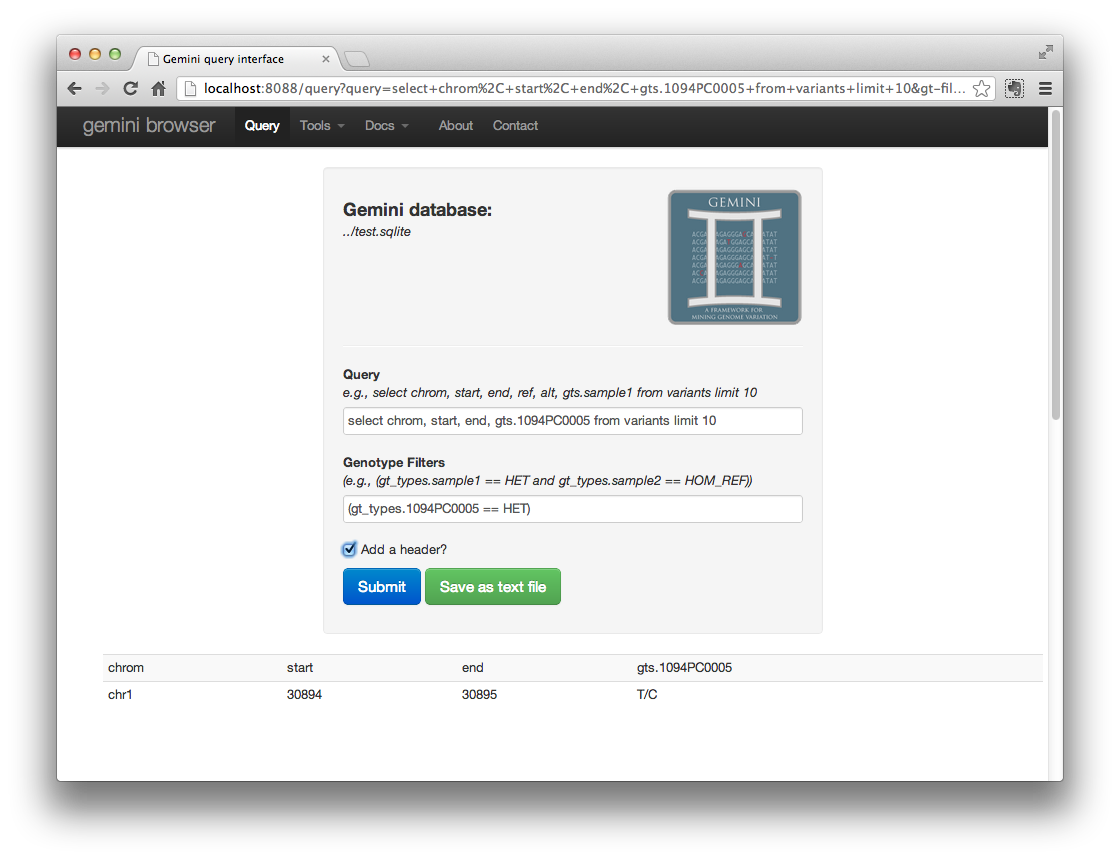
\includegraphics[width=600pt]{browser-query.png}


\section{The Gemini database schema}
\label{content/database_schema::doc}\label{content/database_schema:the-gemini-database-schema}

\subsection{The \texttt{variants} table}
\label{content/database_schema:the-variants-table}

\subsubsection{Core VCF fields}
\label{content/database_schema:core-vcf-fields}
\begin{tabulary}{\linewidth}{|L|L|L|}
\hline
\textbf{
column\_name
} & \textbf{
type
} & \textbf{
notes
}\\\hline

chrom
 & 
STRING
 & 
The chromosome on which the variant resides
\\\hline

start
 & 
INTEGER
 & 
The 0-based start position.
\\\hline

end
 & 
INTEGER
 & 
The 1-based end position.
\\\hline

variant\_id
 & 
INTEGER
 & 
PRIMARY\_KEY
\\\hline

anno\_id
 & 
INTEGER
 & 
Variant transcript number for the most severely affected transcript
\\\hline

ref
 & 
STRING
 & 
Reference allele
\\\hline

alt
 & 
STRING
 & 
Alternate alele for the variant
\\\hline

qual
 & 
INTEGER
 & 
Quality score for the assertion made in ALT
\\\hline

filter
 & 
STRING
 & 
A string of filters passed/failed in variant calling
\\\hline
\end{tabulary}



\subsubsection{Variant and PopGen info}
\label{content/database_schema:variant-and-popgen-info}
\begin{tabular}{|p{0.317\linewidth}|p{0.317\linewidth}|p{0.317\linewidth}|}
\hline
\textbf{} & \textbf{} & \textbf{}\\\hline

type
 & 
STRING
 & 
\begin{DUlineblock}{0em}
\item[] The type of variant.
\item[] Any of: {[}\emph{snp}, \emph{indel}{]}
\end{DUlineblock}
\\\hline

sub\_type
 & 
STRING
 & 
\begin{DUlineblock}{0em}
\item[] The variant sub-type.
\item[] If \code{type} is \emph{snp}:   {[}\emph{ts}, (transition), \emph{tv} (transversion){]}
\item[] If \code{type} is \emph{indel}: {[}\emph{ins}, (insertion), \emph{del} (deletion){]}
\end{DUlineblock}
\\\hline

call\_rate
 & 
FLOAT
 & 
The fraction of samples with a valid genotype
\\\hline

num\_hom\_ref
 & 
INTEGER
 & 
The total number of of homozygotes for the reference (\code{ref}) allele
\\\hline

num\_het
 & 
INTEGER
 & 
The total number of heterozygotes observed.
\\\hline

num\_hom\_alt
 & 
INTEGER
 & 
The total number of homozygotes for the reference (\code{alt}) allele
\\\hline

num\_unknown
 & 
INTEGER
 & 
The total number of of unknown genotypes
\\\hline

aaf
 & 
FLOAT
 & 
The observed allele frequency for the alternate allele
\\\hline

hwe
 & 
FLOAT
 & 
The Chi-square probability of deviation from HWE (assumes random mating)
\\\hline

inbreeding\_coeff
 & 
FLOAT
 & 
The inbreeding co-efficient that expresses the likelihood of effects due to inbreeding
\\\hline

pi
 & 
FLOAT
 & 
The computed nucleotide diversity (pi) for the site
\\\hline
\end{tabular}



\subsubsection{Genotype information}
\label{content/database_schema:genotype-information}
\begin{tabulary}{\linewidth}{|L|L|L|}
\hline
\textbf{} & \textbf{} & \textbf{}\\\hline

gts
 & 
BLOB
 & 
A compressed binary vector of sample genotypes (e.g., ``A/A'', ``A\textbar{}G'', ``G/G'')
\\\hline

gt\_types
 & 
BLOB
 & 
A compressed binary vector of numeric genotype ``types'' (e.g., 0, 1, 2)
\\\hline

gt\_phases
 & 
BLOB
 & 
A compressed binary vector of sample genotype phases (e.g., False, True, False)
\\\hline

gt\_depths
 & 
BLOB
 & 
A compressed binary vector of the depth of aligned sequence observed for each sample
\\\hline
\end{tabulary}



\subsubsection{Gene information}
\label{content/database_schema:gene-information}
\begin{tabular}{|p{0.317\linewidth}|p{0.317\linewidth}|p{0.317\linewidth}|}
\hline
\textbf{} & \textbf{} & \textbf{}\\\hline

gene
 & 
STRING
 & 
Corresponding gene name of the highly affected transcript
\\\hline

transcript
 & 
STRING
 & 
\begin{DUlineblock}{0em}
\item[] The variant transcript that was most severely affected
\item[] (for two equally affected transcripts, either the first
one is selected (VEP) or the protein\_coding biotype is prioritized (snpEff)
\end{DUlineblock}
\\\hline

is\_exonic
 & 
BOOL
 & 
Does the variant affect an exon for \textgreater{}= 1transcript?
\\\hline

is\_coding
 & 
BOOL
 & 
Does the variant fall in a coding region (excl. 3' \& 5' UTRs) for \textgreater{}= 1 transcript?
\\\hline

is\_lof
 & 
BOOL
 & 
Based on the value of the impact col, is the variant LOF for \textgreater{}= transcript?
\\\hline

exon
 & 
STRING
 & 
Exon information for the severely affected transcript
\\\hline

codon\_change
 & 
STRING
 & 
What is the codon change?
\\\hline

aa\_change
 & 
STRING
 & 
What is the amino acid change (for an snp)?
\\\hline

aa\_length
 & 
STRING
 & 
The length of CDS in terms of number of amino acids (\code{only snpEff})
\\\hline

biotype
 & 
STRING
 & 
The `type' of the severely affected transcript (e.g.protein-coding, pseudogene, rRNA etc.) (\code{only snpEff})
\\\hline

impact
 & 
STRING
 & 
The consequence of the most severely affected transcript
\\\hline

impact\_severity
 & 
STRING
 & 
Severity of the highest order observed for the variant
\\\hline

polyphen\_pred
 & 
STRING
 & 
Polyphen predictions for the snps for the severely affected transcript (\code{only VEP})
\\\hline

polyphen\_score
 & 
FLOAT
 & 
Polyphen scores for the severely affected transcript (\code{only VEP})
\\\hline

sift\_pred
 & 
STRING
 & 
SIFT predictions for the snp's for the most severely affected transcript (\code{only VEP})
\\\hline

sift\_score
 & 
FLOAT
 & 
SIFT scores for the predictions (\code{only VEP})
\\\hline

pfam\_domain
 & 
STRING
 & 
Pfam protein domain that the variant affects
\\\hline
\end{tabular}



\subsubsection{Optional VCF INFO fields}
\label{content/database_schema:optional-vcf-info-fields}
\begin{tabulary}{\linewidth}{|L|L|L|}
\hline
\textbf{} & \textbf{} & \textbf{}\\\hline

anc\_allele
 & 
STRING
 & 
The reported ancestral allele if there is one.
\\\hline

rms\_bq
 & 
FLOAT
 & 
The RMS base quality at this position.
\\\hline

cigar
 & 
STRING
 & 
CIGAR string describing how to align an alternate allele to the reference allele.
\\\hline

depth
 & 
INTEGER
 & 
The number of aligned sequence reads that led to this variant call
\\\hline

strand\_bias
 & 
FLOAT
 & 
Strand bias at the variant position
\\\hline

rms\_map\_qual
 & 
FLOAT
 & 
RMS mapping quality, a measure of variance of quality scores
\\\hline

in\_hom\_run
 & 
INTEGER
 & 
Homopolymer runs for the variant allele
\\\hline

num\_mapq\_zero
 & 
INTEGER
 & 
Total counts of reads with mapping quality equal to zero
\\\hline

num\_alleles
 & 
INTEGER
 & 
Total number of alleles in called genotypes
\\\hline

num\_reads\_w\_dels
 & 
FLOAT
 & 
Fraction of reads with spanning deletions
\\\hline

haplotype\_score
 & 
FLOAT
 & 
Consistency of the site with two segregating haplotypes
\\\hline

qual\_depth
 & 
FLOAT
 & 
Variant confidence or quality by depth
\\\hline

allele\_count
 & 
INTEGER
 & 
Allele counts in genotypes
\\\hline

allele\_bal
 & 
FLOAT
 & 
Allele balance for hets
\\\hline

is\_somatic
 & 
BOOL
 & 
Whether the variant is somatically acquired.
\\\hline
\end{tabulary}



\subsubsection{Population information}
\label{content/database_schema:population-information}
\begin{tabular}{|p{0.317\linewidth}|p{0.317\linewidth}|p{0.317\linewidth}|}
\hline
\textbf{} & \textbf{} & \textbf{}\\\hline

in\_dbsnp
 & 
BOOL
 & 
\begin{DUlineblock}{0em}
\item[] Is this variant found in dbSnp (build 135)?
\item[] 0 : Absence of the variant in dbsnp
\item[] 1 : Presence of the variant in dbsnp
\end{DUlineblock}
\\\hline

rs\_ids
 & 
STRING
 & 
\begin{DUlineblock}{0em}
\item[] A comma-separated list of rs ids for variants present in dbsnp
\end{DUlineblock}
\\\hline

in\_hm2
 & 
BOOL
 & 
Whether the variant was part of HapMap2.
\\\hline

in\_hm3
 & 
BOOL
 & 
Whether the variant was part of HapMap3.
\\\hline

in\_esp
 & 
BOOL
 & 
Presence/absence of the variant in the ESP project data
\\\hline

in\_1kg
 & 
BOOL
 & 
Presence/absence of the variant in the 1000 genome project data
\\\hline

aaf\_esp\_ea
 & 
FLOAT
 & 
Minor Allele Frequency of the variant for European Americans in the ESP project
\\\hline

aaf\_esp\_aa
 & 
FLOAT
 & 
Minor Allele Frequency of the variant for African Americans in the ESP project
\\\hline

aaf\_esp\_all
 & 
FLOAT
 & 
Minor Allele Frequency of the variant w.r.t both groups in the ESP project
\\\hline

aaf\_1kg\_amr
 & 
FLOAT
 & 
Allele Frequency of the variant for samples in AMR based on AC/AN (1000g project)
\\\hline

aaf\_1kg\_asn
 & 
FLOAT
 & 
Allele frequency of the variant for samples in ASN based on AC/AN (1000g project)
\\\hline

aaf\_1kg\_afr
 & 
FLOAT
 & 
Allele frequency of the variant for samples in AFR based on AC/AN (1000g project)
\\\hline

aaf\_1kg\_eur
 & 
FLOAT
 & 
Allele Frequency of the variant for samples in EUR based on AC/AN (1000g project)
\\\hline

aaf\_1kg\_all
 & 
FLOAT
 & 
Global allele frequency (based on AC/AN) (1000g project)
\\\hline
\end{tabular}



\subsubsection{Disease phenotype info (from ClinVar).}
\label{content/database_schema:disease-phenotype-info-from-clinvar}
\begin{tabular}{|p{0.317\linewidth}|p{0.317\linewidth}|p{0.317\linewidth}|}
\hline
\textbf{} & \textbf{} & \textbf{}\\\hline

in\_omim
 & 
BOOL
 & 
\begin{DUlineblock}{0em}
\item[] 0 : Absence of the variant in OMIM database
\item[] 1 : Presence of the variant in OMIM database
\end{DUlineblock}
\\\hline

clinvar\_sig
 & 
STRING
 & 
\begin{DUlineblock}{0em}
\item[] The clinical significance scores for each
\item[] of the variant according to ClinVar:
\item[] \emph{unknown}, \emph{untested}, \emph{non-pathogenic}
\item[] \emph{probable-non-pathogenic}, \emph{probable-pathogenic}
\item[] \emph{pathogenic}, \emph{drug-response}, \emph{histocompatibility}
\item[] \emph{other}
\end{DUlineblock}
\\\hline

clinvar\_disease\_name
 & 
STRING
 & 
The name of the disease to which the variant is relevant
\\\hline

clinvar\_dbsource
 & 
STRING
 & 
Variant Clinical Channel IDs
\\\hline

clinvar\_dbsource\_id
 & 
STRING
 & 
The record id in the above database
\\\hline

clinvar\_origin
 & 
STRING
 & 
\begin{DUlineblock}{0em}
\item[] The type of variant.
\item[] Any of:
\item[] \emph{unknown}, \emph{germline}, \emph{somatic},
\item[] \emph{inherited}, \emph{paternal}, \emph{maternal},
\item[] \emph{de-novo}, \emph{biparental}, \emph{uniparental},
\item[] \emph{not-tested}, \emph{tested-inconclusive},
\item[] \emph{other}
\end{DUlineblock}
\\\hline

clinvar\_dsdb
 & 
STRING
 & 
Variant disease database name
\\\hline

clinvar\_dsdbid
 & 
STRING
 & 
Variant disease database ID
\\\hline

clinvar\_disease\_acc
 & 
STRING
 & 
Variant Accession and Versions
\\\hline

clinvar\_in\_locus\_spec\_db
 & 
BOOL
 & 
Submitted from a locus-specific database?
\\\hline

clinvar\_on\_diag\_assay
 & 
BOOL
 & 
Variation is interrogated in a clinical diagnostic assay?
\\\hline
\end{tabular}



\subsubsection{Genome annotations}
\label{content/database_schema:genome-annotations}
\begin{tabular}{|p{0.317\linewidth}|p{0.317\linewidth}|p{0.317\linewidth}|}
\hline
\textbf{} & \textbf{} & \textbf{}\\\hline

exome\_chip
 & 
BOOL
 & 
Whether an SNP is on the Illumina HumanExome Chip
\\\hline

cyto\_band
 & 
STRING
 & 
Chromosomal cytobands that a variant overlaps
\\\hline

rmsk
 & 
STRING
 & 
\begin{DUlineblock}{0em}
\item[] A comma-separated list of RepeatMasker annotations that the variant overlaps.
\item[] Each hit is of the form: \code{name\_class\_family}
\end{DUlineblock}
\\\hline

in\_cpg\_island
 & 
BOOL
 & 
\begin{DUlineblock}{0em}
\item[] Does the variant overlap a CpG island?.
\item[] Based on UCSC: Regulation \textgreater{} CpG Islands \textgreater{} cpgIslandExt
\end{DUlineblock}
\\\hline

in\_segdup
 & 
BOOL
 & 
\begin{DUlineblock}{0em}
\item[] Does the variant overlap a segmental duplication?.
\item[] Based on UCSC: Variation\&Repeats \textgreater{} Segmental Dups \textgreater{} genomicSuperDups track
\end{DUlineblock}
\\\hline

is\_conserved
 & 
BOOL
 & 
\begin{DUlineblock}{0em}
\item[] Does the variant overlap a conserved region?
\item[] Based on the 29-way mammalian conservation study
\end{DUlineblock}
\\\hline

gerp\_bp\_score
 & 
FLOAT
 & 
\begin{DUlineblock}{0em}
\item[] GERP conservation score.
\item[] Only populated if the \code{-{-}load-gerp-bp} option is used when loading.
\item[] Higher scores reflect greater conservation. \textbf{At base-pair resolution}.
\item[] Details: \href{http://mendel.stanford.edu/SidowLab/downloads/gerp/}{http://mendel.stanford.edu/SidowLab/downloads/gerp/}
\end{DUlineblock}
\\\hline

gerp\_element\_pval
 & 
FLOAT
 & 
\begin{DUlineblock}{0em}
\item[] GERP elements P-val
\item[] Lower P-values scores reflect greater conservation. \textbf{Not at base-pair resolution}.
\item[] Details: \href{http://mendel.stanford.edu/SidowLab/downloads/gerp/}{http://mendel.stanford.edu/SidowLab/downloads/gerp/}
\end{DUlineblock}
\\\hline

recomb\_rate
 & 
FLOAT
 & 
\begin{DUlineblock}{0em}
\item[] Returns the mean recombination rate at the variant site
\item[] Based on HapMapII\_GRCh37 genetic map
\end{DUlineblock}
\\\hline
\end{tabular}



\subsubsection{Variant error assessment}
\label{content/database_schema:variant-error-assessment}
\begin{tabular}{|p{0.317\linewidth}|p{0.317\linewidth}|p{0.317\linewidth}|}
\hline
\textbf{} & \textbf{} & \textbf{}\\\hline

grc
 & 
STRING
 & 
\begin{DUlineblock}{0em}
\item[] Association with patch and fix regions from the Genome Reference Consortium:
\item[] \href{http://www.ncbi.nlm.nih.gov/projects/genome/assembly/grc/human/}{http://www.ncbi.nlm.nih.gov/projects/genome/assembly/grc/human/}
\item[] Identifies potential problem regions associated with variant calls.
\item[] Built with \emph{annotation\_provenance/make-ncbi-grc-patches.py}
\end{DUlineblock}
\\\hline

gms\_illumina
 & 
FLOAT
 & 
\begin{DUlineblock}{0em}
\item[] Genome Mappability Scores (GMS) for Illumina error models
\item[] Provides low GMS scores (\textless{} 25.0 in any technology) from:
\item[] \href{http://sourceforge.net/apps/mediawiki/gma-bio/index.php?title=Download\_GMS}{http://sourceforge.net/apps/mediawiki/gma-bio/index.php?title=Download\_GMS}
\item[] \#Download\_GMS\_by\_Chromosome\_and\_Sequencing\_Technology
\item[] Input VCF for annotations prepared with:
\item[] \href{https://github.com/chapmanb/bcbio.variation/blob/master/src/bcbio/variation/utils/gms.clj}{https://github.com/chapmanb/bcbio.variation/blob/master/src/bcbio/variation/utils/gms.clj}
\end{DUlineblock}
\\\hline

gms\_solid
 & 
FLOAT
 & 
Genome Mappability Scores with SOLiD error models
\\\hline

gms\_iontorrent
 & 
FLOAT
 & 
Genome Mappability Scores with IonTorrent error models
\\\hline

in\_cse
 & 
BOOL
 & 
\begin{DUlineblock}{0em}
\item[] Is a variant in an error prone genomic position,
\item[] using CSE: Context-Specific Sequencing Errors
\item[] \href{https://code.google.com/p/discovering-cse/}{https://code.google.com/p/discovering-cse/}
\item[] \href{http://www.biomedcentral.com/1471-2105/14/S5/S1}{http://www.biomedcentral.com/1471-2105/14/S5/S1}
\end{DUlineblock}
\\\hline
\end{tabular}



\subsubsection{ENCODE information}
\label{content/database_schema:encode-information}
\begin{tabular}{|p{0.317\linewidth}|p{0.317\linewidth}|p{0.317\linewidth}|}
\hline
\textbf{} & \textbf{} & \textbf{}\\\hline

encode\_tfbs
 & 
STRING
 & 
\begin{DUlineblock}{0em}
\item[] Comma-separated list of transcription factors that were
\item[] observed by ENCODE to bind DNA in this region.  Each hit in the list is constructed
\item[] as TF\_CELLCOUNT, where:
\item[]
\begin{DUlineblock}{\DUlineblockindent}
\item[] \emph{TF} is the transcription factor name
\item[] \emph{CELLCOUNT} is the number of cells tested that had nonzero signals.
\end{DUlineblock}
\item[] Provenance: wgEncodeRegTfbsClusteredV2 UCSC table
\end{DUlineblock}
\\\hline

encode\_dnaseI\_cell\_count
 & 
INTEGER
 & 
\begin{DUlineblock}{0em}
\item[] Count of cell types that were observed to have DnaseI hypersensitivity.
\end{DUlineblock}
\\\hline

encode\_dnaseI\_cell\_list
 & 
STRING
 & 
\begin{DUlineblock}{0em}
\item[] Comma separated list of cell types that were observed to have DnaseI hypersensitivity.
\item[] Provenance: Thurman, et al, \emph{Nature}, 489, pp. 75-82, 5 Sep. 2012
\end{DUlineblock}
\\\hline

encode\_consensus\_gm12878
 & 
STRING
 & 
\begin{DUlineblock}{0em}
\item[] ENCODE consensus segmentation prediction for GM12878.
\item[] 
\item[] CTCF: CTCF-enriched element
\item[] E:    Predicted enhancer
\item[] PF:   Predicted promoter flanking region
\item[] R:    Predicted repressed or low-activity region
\item[] TSS:  Predicted promoter region including TSS
\item[] T:    Predicted transcribed region
\item[] WE:   Predicted weak enhancer or open chromatin cis-regulatory element
\textbar{} unknown: This region of the genome had no functional prediction.
\end{DUlineblock}
\\\hline

encode\_consensus\_h1hesc
 & 
STRING
 & 
ENCODE consensus segmentation prediction for h1HESC.  See encode\_consseg\_gm12878 for details.
\\\hline

encode\_consensus\_helas3
 & 
STRING
 & 
ENCODE consensus segmentation prediction for Helas3.  See encode\_consseg\_gm12878 for details.
\\\hline

encode\_consensus\_hepg2
 & 
STRING
 & 
ENCODE consensus segmentation prediction for HEPG2.   See encode\_consseg\_gm12878 for details.
\\\hline

encode\_consensus\_huvec
 & 
STRING
 & 
ENCODE consensus segmentation prediction for HuVEC.   See encode\_consseg\_gm12878 for details.
\\\hline

encode\_consensus\_k562
 & 
STRING
 & 
ENCODE consensus segmentation prediction for k562.    See encode\_consseg\_gm12878 for details.
\\\hline
\end{tabular}


\begin{DUlineblock}{0em}
\item[] 
\end{DUlineblock}


\subsection{The \texttt{variant\_impacts} table}
\label{content/database_schema:the-variant-impacts-table}
\begin{tabular}{|p{0.317\linewidth}|p{0.317\linewidth}|p{0.317\linewidth}|}
\hline
\textbf{
column\_name
} & \textbf{
type
} & \textbf{
notes
}\\\hline

variant\_id
 & 
INTEGER
 & 
PRIMARY\_KEY (Foreign key to \emph{variants} table)
\\\hline

anno\_id
 & 
INTEGER
 & 
PRIMARY\_KEY (Based on variant transcripts)
\\\hline

gene
 & 
STRING
 & 
The gene affected by the variant.
\\\hline

transcript
 & 
STRING
 & 
The transcript affected by the variant.
\\\hline

is\_exonic
 & 
BOOL
 & 
Does the variant affect an exon for this transcript?
\\\hline

is\_coding
 & 
BOOL
 & 
Does the variant fall in a coding region (excludes 3' \& 5' UTR's of exons)?
\\\hline

is\_lof
 & 
BOOL
 & 
Based on the value of the impact col, is the variant LOF?
\\\hline

exon
 & 
STRING
 & 
Exon information for the variants that are exonic
\\\hline

codon\_change
 & 
STRING
 & 
What is the codon change?
\\\hline

aa\_change
 & 
STRING
 & 
What is the amino acid change?
\\\hline

aa\_length
 & 
STRING
 & 
The length of CDS in terms of number of amino acids (\code{snpEff only})
\\\hline

biotype
 & 
STRING
 & 
The type of transcript (e.g.protein-coding, pseudogene, rRNA etc.) (\code{SnpEff only})
\\\hline

impact
 & 
STRING
 & 
Impacts due to variation (ref.impact category)
\\\hline

impact\_severity
 & 
STRING
 & 
Severity of the impact based on the impact column value (ref.impact category)
\\\hline

polyphen\_pred
 & 
STRING
 & 
\begin{DUlineblock}{0em}
\item[] Impact of the SNP as given by PolyPhen (\code{VEP only})
\item[] benign, possibly\_damaging, probably\_damaging, unknown
\end{DUlineblock}
\\\hline

polyphen\_scores
 & 
FLOAT
 & 
Polyphen score reflecting severity (higher the impact, \emph{higher} the score) (\code{VEP only})
\\\hline

sift\_pred
 & 
STRING
 & 
\begin{DUlineblock}{0em}
\item[] Impact of the SNP as given by SIFT (\code{VEP only})
\item[] neutral, deleterious
\end{DUlineblock}
\\\hline

sift\_scores
 & 
FLOAT
 & 
SIFT prob. scores reflecting severity (Higher the impact, \emph{lower} the score) (\code{VEP only})
\\\hline
\end{tabular}


\begin{DUlineblock}{0em}
\item[] 
\end{DUlineblock}


\subsection{The \texttt{samples} table}
\label{content/database_schema:the-samples-table}
\begin{tabulary}{\linewidth}{|L|L|L|}
\hline
\textbf{
column name
} & \textbf{
type
} & \textbf{
notes
}\\\hline

sample\_id
 & 
INTEGER
 & 
PRIMARY\_KEY
\\\hline

name
 & 
STRING
 & 
Sample names
\\\hline

family\_id
 & 
INTEGER
 & 
Family ids for the samples {[}User defined, default: NULL{]}
\\\hline

paternal\_id
 & 
INTEGER
 & 
Paternal id for the samples {[}User defined, default: NULL{]}
\\\hline

maternal\_id
 & 
INTEGER
 & 
Maternal id for the samples {[}User defined, default: NULL{]}
\\\hline

sex
 & 
STRING
 & 
Sex of the sample {[}User defined, default: NULL{]}
\\\hline

phenotype
 & 
STRING
 & 
The associated sample phenotype {[}User defined, default: NULL{]}
\\\hline

ethnicity
 & 
STRING
 & 
The ethnic group to which the sample belongs {[}User defined, default: NULL{]}
\\\hline
\end{tabulary}


\begin{DUlineblock}{0em}
\item[] 
\end{DUlineblock}


\subsection{Details of the \texttt{impact} and \texttt{impact\_severity} columns}
\label{content/database_schema:details-of-the-impact-and-impact-severity-columns}
\begin{tabular}{|p{0.475\linewidth}|p{0.475\linewidth}|}
\hline
\textbf{
impact severity
} & \textbf{
impacts
}\\\hline

HIGH
 & \begin{itemize}
\item {} 
exon\_deleted

\item {} 
frame\_shift

\item {} 
splice\_acceptor

\item {} 
splice\_donor

\item {} 
start\_loss

\item {} 
stop\_gain

\item {} 
stop\_loss

\item {} 
non\_synonymous\_start

\end{itemize}
\\\hline

MED
 & \begin{itemize}
\item {} 
non\_syn\_coding

\item {} 
inframe\_codon\_gain

\item {} 
inframe\_codon\_loss

\item {} 
inframe\_codon\_change

\item {} 
codon\_change\_del

\item {} 
codon\_change\_ins

\item {} 
UTR\_5\_del

\item {} 
UTR\_3\_del

\item {} 
other\_splice\_variant

\item {} 
mature\_miRNA

\item {} 
regulatory\_region

\item {} 
TF\_binding\_site

\item {} 
regulatory\_region\_ablation

\item {} 
regulatory\_region\_amplification

\item {} 
TFBS\_ablation

\item {} 
TFBS\_amplification

\end{itemize}
\\\hline

LOW
 & \begin{itemize}
\item {} 
synonymous\_stop

\item {} 
synonymous\_coding

\item {} 
UTR\_5\_prime

\item {} 
UTR\_3\_prime

\item {} 
intron

\item {} 
CDS

\item {} 
upstream

\item {} 
downstream

\item {} 
intergenic

\item {} 
intragenic

\item {} 
gene

\item {} 
transcript

\item {} 
exon

\item {} 
start\_gain

\item {} 
synonymous\_start

\item {} 
intron\_conserved

\item {} 
nc\_transcript

\item {} 
NMD\_transcript

\item {} 
transcript\_codon\_change

\item {} 
incomplete\_terminal\_codon

\item {} 
nc\_exon

\item {} 
transcript\_ablation

\item {} 
transcript\_amplification

\item {} 
feature elongation

\item {} 
feature truncation

\end{itemize}
\\\hline
\end{tabular}



\subsection{The \texttt{resources} table}
\label{content/database_schema:the-resources-table}
Establishes provenance of annotation resources used to create a Gemini database.

\begin{tabulary}{\linewidth}{|L|L|L|}
\hline
\textbf{
column name
} & \textbf{
type
} & \textbf{
notes
}\\\hline

name
 & 
STRING
 & 
Name of the annotation type
\\\hline

resource
 & 
STRING
 & 
Filename of the resource, with version information
\\\hline
\end{tabulary}



\subsection{The \texttt{version} table}
\label{content/database_schema:the-version-table}
Establishes which version of \code{gemini} was used to create a database.

\begin{tabulary}{\linewidth}{|L|L|L|}
\hline
\textbf{
column name
} & \textbf{
type
} & \textbf{
notes
}\\\hline

version
 & 
STRING
 & 
What version of gemini was used to create the DB.
\\\hline
\end{tabulary}



\section{Using the GEMINI API}
\label{content/api:using-the-gemini-api}\label{content/api::doc}\label{content/api:module-gemini}\index{gemini (module)}

\subsection{The GeminiQuery class}
\label{content/api:the-geminiquery-class}\index{GeminiQuery (class in gemini)}

\begin{fulllineitems}
\phantomsection\label{content/api:gemini.GeminiQuery}\pysiglinewithargsret{\strong{class }\code{gemini.}\bfcode{GeminiQuery}}{\emph{db}}{}
An interface to submit queries to an existing Gemini database
and iterate over the results of the query.

We create a GeminiQuery object by specifying database to which to
connect:

\begin{Verbatim}[commandchars=\\\{\}]
\PYG{k+kn}{from} \PYG{n+nn}{gemini} \PYG{k+kn}{import} \PYG{n}{GeminiQuery}
\PYG{n}{gq} \PYG{o}{=} \PYG{n}{GeminiQuery}\PYG{p}{(}\PYG{l+s}{"}\PYG{l+s}{my.db}\PYG{l+s}{"}\PYG{p}{)}
\end{Verbatim}

We can then issue a query against the database and iterate through
the results by using the \code{run()} method:

\begin{Verbatim}[commandchars=\\\{\}]
\PYG{n}{gq}\PYG{o}{.}\PYG{n}{run}\PYG{p}{(}\PYG{l+s}{"}\PYG{l+s}{select chrom, start, end from variants}\PYG{l+s}{"}\PYG{p}{)}
\PYG{k}{for} \PYG{n}{row} \PYG{o+ow}{in} \PYG{n}{gq}\PYG{p}{:}
    \PYG{k}{print} \PYG{n}{row}
\end{Verbatim}

Instead of printing the entire row, one access print specific columns:

\begin{Verbatim}[commandchars=\\\{\}]
\PYG{n}{gq}\PYG{o}{.}\PYG{n}{run}\PYG{p}{(}\PYG{l+s}{"}\PYG{l+s}{select chrom, start, end from variants}\PYG{l+s}{"}\PYG{p}{)}
\PYG{k}{for} \PYG{n}{row} \PYG{o+ow}{in} \PYG{n}{gq}\PYG{p}{:}
    \PYG{k}{print} \PYG{n}{row}\PYG{p}{[}\PYG{l+s}{'}\PYG{l+s}{chrom}\PYG{l+s}{'}\PYG{p}{]}
\end{Verbatim}

Also, all of the underlying numpy genotype arrays are
always available:

\begin{Verbatim}[commandchars=\\\{\}]
\PYG{n}{gq}\PYG{o}{.}\PYG{n}{run}\PYG{p}{(}\PYG{l+s}{"}\PYG{l+s}{select chrom, start, end from variants}\PYG{l+s}{"}\PYG{p}{)}
\PYG{k}{for} \PYG{n}{row} \PYG{o+ow}{in} \PYG{n}{gq}\PYG{p}{:}
    \PYG{n}{gts} \PYG{o}{=} \PYG{n}{row}\PYG{o}{.}\PYG{n}{gts}
    \PYG{k}{print} \PYG{n}{row}\PYG{p}{[}\PYG{l+s}{'}\PYG{l+s}{chrom}\PYG{l+s}{'}\PYG{p}{]}\PYG{p}{,} \PYG{n}{gts}
    \PYG{c}{\PYGZsh{} yields "chr1" ['A/G' 'G/G' ... 'A/G']}
\end{Verbatim}

The \code{run()} methods also accepts genotype filter:

\begin{Verbatim}[commandchars=\\\{\}]
query = "select chrom, start, end" from variants"
gt\_filter = "gt\_types.NA20814 == HET"
gq.run(query)
for row in gq:
    print row
\end{Verbatim}

Lastly, one can use the \code{sample\_to\_idx} and \code{idx\_to\_sample}
dictionaries to gain access to sample-level genotype information
either by sample name or by sample index:

\begin{Verbatim}[commandchars=\\\{\}]
\PYG{c}{\PYGZsh{} grab dict mapping sample to genotype array indices}
\PYG{n}{smp2idx} \PYG{o}{=} \PYG{n}{gq}\PYG{o}{.}\PYG{n}{sample\PYGZus{}to\PYGZus{}idx}

\PYG{n}{query}  \PYG{o}{=} \PYG{l+s}{"}\PYG{l+s}{select chrom, start, end from variants}\PYG{l+s}{"}
\PYG{n}{gt\PYGZus{}filter}  \PYG{o}{=} \PYG{l+s}{"}\PYG{l+s}{gt\PYGZus{}types.NA20814 == HET}\PYG{l+s}{"}
\PYG{n}{gq}\PYG{o}{.}\PYG{n}{run}\PYG{p}{(}\PYG{n}{query}\PYG{p}{,} \PYG{n}{gt\PYGZus{}filter}\PYG{p}{)}

\PYG{c}{\PYGZsh{} print a header listing the selected columns}
\PYG{k}{print} \PYG{n}{gq}\PYG{o}{.}\PYG{n}{header}
\PYG{k}{for} \PYG{n}{row} \PYG{o+ow}{in} \PYG{n}{gq}\PYG{p}{:}
    \PYG{c}{\PYGZsh{} access a NUMPY array of the sample genotypes.}
    \PYG{n}{gts} \PYG{o}{=} \PYG{n}{row}\PYG{p}{[}\PYG{l+s}{'}\PYG{l+s}{gts}\PYG{l+s}{'}\PYG{p}{]}
    \PYG{c}{\PYGZsh{} use the smp2idx dict to access sample genotypes}
    \PYG{n}{idx} \PYG{o}{=} \PYG{n}{smp2idx}\PYG{p}{[}\PYG{l+s}{'}\PYG{l+s}{NA20814}\PYG{l+s}{'}\PYG{p}{]}
    \PYG{k}{print} \PYG{n}{row}\PYG{p}{,} \PYG{n}{gts}\PYG{p}{[}\PYG{n}{idx}\PYG{p}{]}
\end{Verbatim}
\index{run() (gemini.GeminiQuery method)}

\begin{fulllineitems}
\phantomsection\label{content/api:gemini.GeminiQuery.run}\pysiglinewithargsret{\bfcode{run}}{\emph{query}, \emph{gt\_filter=None}, \emph{show\_variant\_samples=False}}{}
Execute a query against a Gemini database. The user may
specify:
\begin{enumerate}
\item {} 
(reqd.) an SQL \emph{query}.

\item {} 
(opt.) a genotype filter.

\end{enumerate}

\end{fulllineitems}

\index{header (gemini.GeminiQuery attribute)}

\begin{fulllineitems}
\phantomsection\label{content/api:gemini.GeminiQuery.header}\pysigline{\bfcode{header}}
Return a header describing the columns that
were selected in the query issued to a GeminiQuery object.

\end{fulllineitems}

\index{sample2index (gemini.GeminiQuery attribute)}

\begin{fulllineitems}
\phantomsection\label{content/api:gemini.GeminiQuery.sample2index}\pysigline{\bfcode{sample2index}}
Return a dictionary mapping sample names to
genotype array offsets:

\begin{Verbatim}[commandchars=\\\{\}]
\PYG{n}{gq} \PYG{o}{=} \PYG{n}{GeminiQuery}\PYG{p}{(}\PYG{l+s}{"}\PYG{l+s}{my.db}\PYG{l+s}{"}\PYG{p}{)}
\PYG{n}{s2i} \PYG{o}{=} \PYG{n}{gq}\PYG{o}{.}\PYG{n}{sample2index}

\PYG{k}{print} \PYG{n}{s2i}\PYG{p}{[}\PYG{l+s}{'}\PYG{l+s}{NA20814}\PYG{l+s}{'}\PYG{p}{]}
\PYG{c}{\PYGZsh{} yields 1088}
\end{Verbatim}

\end{fulllineitems}

\index{index2sample (gemini.GeminiQuery attribute)}

\begin{fulllineitems}
\phantomsection\label{content/api:gemini.GeminiQuery.index2sample}\pysigline{\bfcode{index2sample}}
Return a dictionary mapping sample names to
genotype array offsets:

\begin{Verbatim}[commandchars=\\\{\}]
\PYG{n}{gq} \PYG{o}{=} \PYG{n}{GeminiQuery}\PYG{p}{(}\PYG{l+s}{"}\PYG{l+s}{my.db}\PYG{l+s}{"}\PYG{p}{)}
\PYG{n}{i2s} \PYG{o}{=} \PYG{n}{gq}\PYG{o}{.}\PYG{n}{index2sample}

\PYG{k}{print} \PYG{n}{i2s}\PYG{p}{[}\PYG{l+m+mi}{1088}\PYG{p}{]}
\PYG{c}{\PYGZsh{} yields "NA20814"}
\end{Verbatim}

\end{fulllineitems}


\end{fulllineitems}



\section{Acknowledgements}
\label{content/acknowledgements:acknowledgements}\label{content/acknowledgements::doc}
GEMINI is developed by Uma Paila and Aaron Quinlan in the
\href{http://quinlanlab.org/}{Quinlan laboratory} at the University of Virginia.
Substantial contributions to the design, functionality, and code base have been
made by the following:
\begin{itemize}
\item {} 
Brad Chapman, HSPH

\item {} 
Rory Kirchner, HSPH

\item {} 
Oliver Hofmann, HSPH

\end{itemize}


\section{Release History}
\label{content/history::doc}\label{content/history:release-history}

\subsection{0.3.0b}
\label{content/history:b}\begin{enumerate}
\item {} 
Improved speed for adding custom annotations.

\item {} 
Added GERP conserved elements.

\item {} 
Optionally addition of GERP conservation scores at base pair resolution.

\item {} 
Move annotation files to Amazon S3.

\end{enumerate}


\section{F.A.Q.}
\label{content/faq::doc}\label{content/faq:f-a-q}

\subsection{Does GEMINI work with non-human genomes?}
\label{content/faq:does-gemini-work-with-non-human-genomes}
Currently, no.  However, we recognize that the GEMINI framework is suitable to
genetic research in other organisms. This may be a focus of future work.


\subsection{What versions of the human genome does GEMINI support?}
\label{content/faq:what-versions-of-the-human-genome-does-gemini-support}
Currently, we support solely build 37 of the human genome (a.k.a, hg19). We intend to support forthcoming versions of the human genome in future releases.


\subsection{How can I use PLINK files with GEMINI?}
\label{content/faq:how-can-i-use-plink-files-with-gemini}
Many datasets, especially those derived from GWAS studies, are based on SNP
genotyping arrays, and are thus stored in the  standard PLINK formats.
While GEMINI only supports VCF input files, it is relatively straightforward to
convert PLINK datasets to VCF with the PLINK/SEQ toolkit.

1. First, load the PLINK BED file into a new PLINK/SEQ project using the instructions
found in the ``Load a PLINK binary fileset'' section \href{http://atgu.mgh.harvard.edu/plinkseq/input.shtml\#plink}{here}.

2. Next, use PLINK/SEQ to convert the project to VCF using the instructions found
\href{http://atgu.mgh.harvard.edu/plinkseq/output.shtml\#vcf}{here}.

At this point, you should have a VCF file that is compatible with GEMINI.

Alternatively, in his \href{https://github.com/chapmanb/bcbio-nextgen}{bcbio} project, Brad Chapman has written a convenient
\href{https://github.com/chapmanb/bcbio-nextgen/blob/master/scripts/plink\_to\_vcf.py}{script} for directly converting PLINK files to VCF.  Below is an example of how to use
this script.

\begin{Verbatim}[commandchars=\\\{\}]
\PYG{n+nv}{\PYGZdl{} }plink\PYGZus{}to\PYGZus{}vcf.py \PYGZlt{}ped file\PYGZgt{} \PYGZlt{}map file\PYGZgt{} \PYGZlt{}UCSC reference file in 2bit format\PYG{o}{)}
\end{Verbatim}


\renewcommand{\indexname}{Python Module Index}
\begin{theindex}
\def\bigletter#1{{\Large\sffamily#1}\nopagebreak\vspace{1mm}}
\bigletter{g}
\item {\texttt{gemini}}, \pageref{content/api:module-gemini}
\end{theindex}

\renewcommand{\indexname}{Index}
\printindex
\end{document}
